\documentclass{article}

% NeurIPS 2025 style: [preprint] for public dissemination;
% switch to \usepackage{neurips_2025} for anonymous double-blind submission.
\PassOptionsToPackage{numbers,sort&compress}{natbib}
\usepackage[preprint]{neurips_2025}

\usepackage[utf8]{inputenc}
\usepackage[T1]{fontenc}
\usepackage{microtype}
\usepackage{amsmath,amssymb,amsthm,mathtools,bm}
\usepackage{booktabs}
\usepackage{graphicx}
\usepackage{xcolor}
\usepackage{enumitem}
\usepackage[ruled,vlined,linesnumbered]{algorithm2e}
\usepackage[colorlinks=true,linkcolor=blue!60!black,citecolor=green!50!black,urlcolor=blue!70!black]{hyperref}
\usepackage[capitalize,noabbrev]{cleveref}

\graphicspath{{figures/}{../results/figures/}}

\crefname{algocf}{Algorithm}{Algorithms}
\Crefname{algocf}{Algorithm}{Algorithms}

\theoremstyle{plain}
\newtheorem{theorem}{Theorem}
\newtheorem{proposition}{Proposition}
\newtheorem{lemma}{Lemma}
\newtheorem{corollary}{Corollary}

\theoremstyle{definition}
\newtheorem{definition}{Definition}
\newtheorem{assumption}{Assumption}

\theoremstyle{remark}
\newtheorem{remark}{Remark}

\newcommand{\R}{\mathbb{R}}
\newcommand{\E}{\mathbb{E}}
\newcommand{\Prob}{\mathbb{P}}
\newcommand{\Var}{\operatorname{Var}}
\newcommand{\Cov}{\operatorname{Cov}}
\newcommand{\KL}{\operatorname{kl}}
\newcommand{\DKL}{D_{\mathrm{KL}}}
\newcommand{\TV}{\operatorname{TV}}
\newcommand{\SNR}{\operatorname{SNR}}
\newcommand{\logit}{\operatorname{logit}}
\newcommand{\ind}{\mathbf{1}}
\newcommand{\Fmix}{F_{\mathrm{mix}}}
\newcommand{\barFmix}{\bar{F}_{\mathrm{mix}}}
\newcommand{\fmix}{f_{\mathrm{mix}}}

\title{Joint Calibration--Compute Limits of Test-Time Scaling:\\
Minimax Theory, Prompt Heterogeneity, and Risk-Controlled Verifier Selection}

\author{%
  Test-Time Scaling Theory Working Group \\
  \texttt{https://github.com/6Riemann9/test-time-scaling-theory}
}

\begin{document}

\maketitle

\begin{abstract}
Best-of-$N$ ($\mathrm{BoN}$) test-time scaling improves reasoning accuracy only while extreme verifier scores stay aligned with correctness; when wrong-answer tails are heavier or spike-contaminated, larger compute $N$ degrades accuracy. Although post-hoc calibration restores monotonicity for fixed prompts, real deployments face finite offline labels ($M$), finite online unlabeled candidates ($N$), and cross-prompt difficulty and score-scale heterogeneity. Within a unified two-level hierarchical framework, we establish three complementary limits. First, over a uniformly regular $\beta$-smooth peak class, joint minimax simple regret decouples additively as $\Theta\!\big((\frac{\ln M}{M})^{\frac{\beta}{2\beta+1}} + N^{-\beta}\big)$, attained by an $N$-agnostic equal-frequency $\mathrm{KL\text{-}LCB}$ rule with balance threshold $N_{\mathrm{balance}}(M) \asymp (M/\ln M)^{\frac{1}{2\beta+1}}$ and extended to unknown marginals for all $\beta > 0$ via sample-split Uniform spacings. Second, under hierarchical heterogeneity, we derive an exact Simpson derivative decomposition with grid-free masking, prove that online sample Z-scores converge uniformly at $O_p(\sqrt{(\ln N)/N})$ yet suffer an affine-invariant asymptotic ceiling loss whenever unsolvable prompts exist ($\pi_0 > 0$), and bound a three-branch holdout selector ($\mathrm{Hybrid\text{-}Fixed}$). Third, we characterize multi-verifier Gaussian spectral paths and Copula tail boundaries. Across five public LLM benchmarks (over $1.1\times 10^6$ trajectories), $\mathrm{Hybrid\text{-}Fixed}$ avoids cross-domain Simpson confounding ($+2.41\,\mathrm{pp}$, $p_t=0.0050$ on \texttt{S3}; $+1.83\,\mathrm{pp}$, $p_t=0.0120$ on \texttt{RB2}), sidesteps within-prompt Z-score ceiling drops ($-2.91$ to $-9.16\,\mathrm{pp}$), and prevents tail-contamination collapse ($+42.29\,\mathrm{pp}$).
\end{abstract}

\section{Introduction}
\label{sec:intro}

Sampling $N$ candidate solutions from a language model and selecting one via a reward model (RM) or process reward model (PRM) improves reasoning without updating model weights \citep{gao2023scaling,brown2024large,snell2024scaling}. However, standard Best-of-$N$ ($\mathrm{BoN}$) probes the extreme upper tail $S_{(N)} = \max_{1\le i\le N} S_i$, where heavy or spike-contaminated wrong-answer tails trigger \emph{verifier overoptimization}: accuracy peaks at a finite budget and decays toward zero as $N$ grows \citep{gao2023scaling,stroebl2024inference,huang2025best,dorner2025roc,yano2026tail,gui2026whether}.

Replacing raw score maximization with the fixed-prompt Bayesian posterior $q(s) = \Prob(Y=1 \mid S=s)$ restores monotone scaling in the population limit. Yet deploying calibrated $\mathrm{BoN}$ under finite resources and real multi-domain workloads raises three coupled statistical questions:
\begin{enumerate}[leftmargin=1.8em,itemsep=2pt]
    \item \textbf{Joint Calibration--Compute Minimax Limits:} Given $M$ offline labeled pairs $\mathcal{D}_M \sim P^{\otimes M}$ and $N$ online unlabeled candidates $S_{1:N} \sim \Fmix^{\otimes N}$, what is the minimax regret $\mathcal{R}^*(M, N)$, and when does label scarcity bottleneck compute scaling?
    \item \textbf{Hierarchical Prompt Heterogeneity and Sample Standardization:} When prompts $X \sim \mathcal{P}_X$ vary in solvability $p(X)$ and score affine shifts $(b(X), a(X))$, when does pooled calibration fail via Simpson confounding, and does online prompt-wise Z-standardization $Z_{i,N}$ cure heterogeneity without distorting extreme tails?
    \item \textbf{Risk-Controlled Selection and Ensembling:} How can a system select safely among raw, pooled, and Z-standardized predictors using finite holdout validation, defend against unseen distribution shift, and exploit correlation structure across multiple RMs?
\end{enumerate}

\paragraph{Contributions and Attribution Boundaries.}
We present two primary theoretical pillars, a supplementary multi-verifier pillar, and a protocol-aligned empirical audit across five public benchmarks (\Cref{fig:overview}):
\begin{itemize}[leftmargin=1.6em,itemsep=3pt]
    \item \textbf{Joint $(M,N)$ Minimax Regret and All-$\beta$ Spacings (\Cref{sec:minimax}).} Defining a uniformly regular $\beta$-smooth peak class $\mathcal{F}_\beta^{\mathrm{unif}}(C_1, f_{\min}, \eta_0)$ ($\beta > 0$), \Cref{thm:joint-minimax} proves that a static $N$-agnostic equal-frequency $\mathrm{KL\text{-}LCB}$ rule achieves rate $\Theta\big((\frac{\ln M}{M})^{\frac{\beta}{2\beta+1}} + N^{-\beta}\big)$ across all $(M,N)$ without $(\ln N)^\beta$ coupling inflation, yielding the calibration--compute balance threshold $N_{\mathrm{balance}}(M) \asymp (M/\ln M)^{\frac{1}{2\beta+1}}$. For unknown marginals and all $\beta > 0$, \Cref{prop:spacings} (\Cref{alg:split-kl-lcb}) uses sample-split Pyke spacings to establish multiplicative bin-mass concentration $\hat{\pi}_k \in [\frac{1}{2K}, \frac{143}{72K})$, bypassing additive Dvoretzky--Kiefer--Wolfowitz (DKW) failure when $0 < \beta \le 1/2$.
    \item \textbf{Hierarchical Simpson Masking, Online Sample-$Z_{i,N}$ Inversion, and Holdout Gating (\Cref{sec:heterogeneity}).} \Cref{thm:simpson} decomposes the pooled posterior slope and constructs a grid-free analytical two-stratum masking example on $[3.5, 4.2]$. \Cref{thm:zscore-n2} establishes $N=2$ rank-only bounds and bidirectional order-reversal conditions. \Cref{thm:sample-z-ceiling} proves that whenever unsolvable prompts occur ($\pi_0 > 0$), online sample Z-scores satisfy $\max_{1\le i\le N}|Z_{i,N} - Z_i^*(X)| = O_p(\sqrt{(\ln N)/N})$ and suffer an affine-invariant asymptotic ceiling loss below $\mathrm{Raw\text{-}BoN}$. \Cref{prop:hybrid} (\Cref{alg:hybrid-fixed}) bounds the risk of three-branch holdout gating and post-selection refitting.
    \item \textbf{Multi-Verifier Correlation, Single-Verifier Scope, and Empirical Audit (\Cref{sec:ensemble,sec:experiments,sec:discussion}).} \Cref{sec:ensemble} establishes the $\mathrm{Safe\text{-}Fisher}$ spectral path, QDA $N^{-2/K}$ scaling, and degenerate-KKT Gaussian/Copula $\mathrm{Min\text{-}Ensemble}$ tail exponents. Single-verifier preliminaries remain in \Cref{app:preliminaries} without priority claims, while \Cref{sec:experiments} audits quantile protocols, disjoint 50/20/30 studentized $t$-tests, natural overoptimization on \texttt{college\_math}, four-regime contamination shift, and multi-RM correlations.
\end{itemize}

\paragraph{Organization.}
Building on the three motivating questions in \Cref{sec:intro}, \Cref{sec:related} situates our results within test-time scaling, nonparametric extrema estimation, and offline pessimism. \Cref{sec:model} formalizes the two-level model, \Cref{sec:minimax,sec:heterogeneity} present the main minimax and heterogeneity theorems alongside \Cref{alg:split-kl-lcb,alg:hybrid-fixed}, \Cref{sec:ensemble} develops multi-verifier theory, \Cref{sec:experiments} details empirical verification, and \Cref{sec:discussion} covers limitations, broader impact, and reproducibility (supported by \Cref{app:preliminaries,app:minimax,app:heterogeneity,app:ensemble,app:index,app:checklist}).

\section{Related Work}
\label{sec:related}

\paragraph{Test-Time Scaling and Verifier Overoptimization.}
Empirical scaling studies demonstrate both the power of repeated sampling \citep{brown2024large,snell2024scaling} and Goodhart overoptimization against learned RMs \citep{gao2023scaling}. Recent analyses formalize single-verifier scaling limits via binary false positives \citep{stroebl2024inference}, instance-level ROC geometry \citep{dorner2025roc}, univariate extreme-value tail competition \citep{yano2026tail}, and Beta quantile tail-calibration signals \citep{gui2026whether}, alongside practical calibrated $\mathrm{BoN}$ \citep{tang2025carbon}, sample-based $\mathrm{BoN}$ policy evaluation \citep{schweisthal2026efficient}, and pessimistic rejection sampling \citep{huang2025best}. Our work unifies single-verifier preliminaries (\Cref{app:preliminaries}) and shifts focus to the unexplored statistical bottlenecks of \emph{coupled} finite $(M, N)$ calibration, cross-prompt hierarchical pooling, and multi-verifier correlation structure.

\paragraph{Nonparametric Extrema Estimation and Offline Pessimism.}
At $N = \infty$, our offline rate $(\frac{\ln M}{M})^{\frac{\beta}{2\beta+1}}$ aligns with classical passive kernel and Fano lower bounds for estimating regression maxima and modes \citep{muller1985kernel,romano1988weak,tsybakov2009introduction}, as well as the first-stage non-adaptive benchmark highlighted by \citet{belitser2012optimal}. Active two-stage zooming \citep{belitser2012optimal}, selective label querying \citep{minsker2013estimation}, and continuum-armed bandits \citep{bubeck2011xarmed} accelerate convergence by querying adaptively near peaks. In offline test-time calibration, however, $\mathcal{D}_M \sim P^{\otimes M}$ is passively generated and online selection is confined to $N$ random unlabeled candidates $S_{1:N}$, adding the irreducible $N^{-\beta}$ order-statistic spacing term. Our binned estimator adapts classical $\mathrm{KL\text{-}UCB/LCB}$ \citep{garivier2011kl} and offline pessimism \citep{jin2021pessimism} to unknown marginals via Pyke's Gamma spacings \citep{pyke1965spacings}.

\paragraph{Multi-Verifier Ensembles, Prompt Heterogeneity, and Inference.}
Ensembling multiple RMs via worst-case optimization or weight averaging mitigates overoptimization \citep{coste2024reward,rame2024warm}, but existing theory lacks exact phase boundaries for negative-weight noise cancellation and weakly active multivariate Gaussian/Copula extremes \citep{savage1962mills,hashorva2003multivariate,tankov2016tails,das2024heavy}. On evaluation methodology, \citet{nadeau2003inference} establish that cross-validation fold overlap underestimates variance; we therefore adopt disjoint single-split holdout testing as primary inference and reserve \citet{phipson2010permutation} exactness corrections for auxiliary permutation checks.

\section{Hierarchical Probabilistic Model and Scope Delineation}
\label{sec:model}

We model test-time reasoning on a probability space $(\Omega, \mathcal{F}, \Prob)$ with a two-level hierarchy (\Cref{fig:overview}(a)):
\begin{enumerate}[leftmargin=1.8em,itemsep=2pt]
    \item A prompt $X \sim \mathcal{P}_X$ induces a latent prior correctness rate $p(X) := \Prob(Y = 1 \mid X) \in [0, 1]$.
    \item Conditional on $X$, a generator draws $N \ge 1$ i.i.d.\ candidates $\{(Y_i, S_i)\}_{i=1}^N \mid X \stackrel{\mathrm{i.i.d.}}{\sim} P_{Y, S \mid X}$, with correctness $Y_i \in \{0, 1\}$, verifier score $S_i \in \R$ (or $\mathbf{S}_i \in \R^K$ in \Cref{sec:ensemble}), and class CDFs $F_{c, X}(s) := \Prob(S_i \le s \mid Y_i = c, X)$ for $c \in \{0, 1\}$.
\end{enumerate}

\begin{figure}[t]
\centering
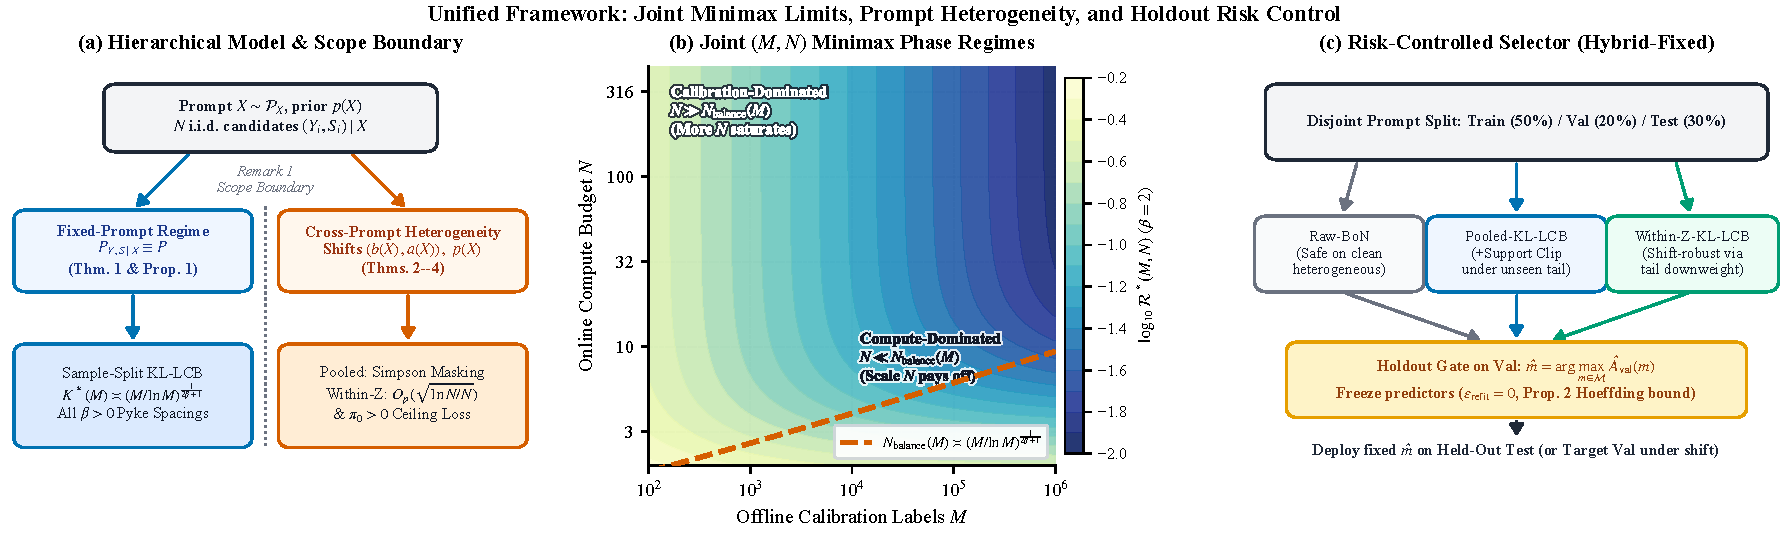
\includegraphics[width=\textwidth]{fig1_framework_overview}
\caption{\textbf{Framework overview.} \textbf{(a)} Two-level generative--verification hierarchy separating fixed-prompt calibration (\Cref{sec:minimax}) from cross-prompt pooling (\Cref{sec:heterogeneity}). \textbf{(b)} Joint $(M, N)$ minimax regret surface ($\beta=2$) and balance boundary $N_{\mathrm{balance}}(M)$. \textbf{(c)} Three-branch holdout risk-control gate ($\mathrm{Hybrid\text{-}Fixed}$, \Cref{alg:hybrid-fixed}).}
\label{fig:overview}
\end{figure}

\begin{remark}[Scope Boundary: Fixed-Prompt Guarantees vs.\ Cross-Prompt Pooling]
\label{rem:scope}
In \Cref{sec:minimax,sec:ensemble} (and \Cref{app:preliminaries}), we condition on a fixed prompt $X = x$ (or a homogeneous population $P_{Y,S\mid X} \equiv P$), suppressing $X$ to write $p \in (0, 1)$, $\Fmix(s) = p F_1(s) + (1-p)F_0(s)$, $\barFmix = 1 - \Fmix$, and posterior $q(s) = \Prob(Y=1 \mid S=s) = \frac{d(p\mu_1)}{d\mu_{\mathrm{mix}}}(s)$. Under fixed $P$, candidates are i.i.d.\ and minimax calibration guarantees hold unconditionally. Across heterogeneous prompts, candidates are only conditionally independent and $q_{\mathrm{pool}}(s) = \E[q_X(s) \mid S=s]$ departs from $q_X(s)$; \Cref{sec:heterogeneity} explicitly analyzes this mismatch.
\end{remark}

Given $S_{1:N}$, standard $\mathrm{BoN}$ selects uniformly from $\mathcal{I}_{\max} := \{i : S_i = S_{(N)}\}$, achieving accuracy $P_{\mathrm{BoN}}(N) := \Prob(Y_{i^*} = 1)$. By \Cref{thm:app-pit} (\Cref{app:preliminaries}), for any distribution with countable tie atoms $\mathcal{A}$ and left-continuous quantile $\Fmix^{-1}(u) := \inf\{x : \Fmix(x) \ge u\}$,
\begin{equation}
\label{eq:pit-exact}
P_{\mathrm{BoN}}(N) = \int_{\R} q(x)\, d\big([\Fmix(x)]^N\big) = \int_0^1 q\big(\Fmix^{-1}(v^{1/N})\big)\, dv.
\end{equation}
If positive densities $f_1, f_0$ satisfy $\lim_{x \uparrow x_R} f_1(x)/f_0(x) = 0$ (including heteroscedastic Gaussians $\sigma_0 > \sigma_1$ and contaminated wrong-answer tails), $\lim_{N\to\infty} P_{\mathrm{BoN}}(N) = 0$ (\Cref{thm:app-collapse}). Maximizing the true single-prompt posterior $Q_i = q(S_i)$ instead yields monotone convergence $P_{\mathrm{Cal\text{-}BoN}}(N) = \E[Q_{(N)}] \uparrow \operatorname{ess\,sup} q(S)$ (\Cref{thm:app-cal}).

\section{Joint Calibration--Compute Minimax Theory}
\label{sec:minimax}

Condition on a fixed prompt distribution $P$ (\Cref{rem:scope}). An offline labeled dataset $\mathcal{D}_M = \{(\tilde{S}_j, \tilde{Y}_j)\}_{j=1}^M \sim P^{\otimes M}$ is observed passively prior to drawing $N$ online unlabeled test candidates $S_{1:N} \sim \Fmix^{\otimes N}$. Partitioning $\R$ into $K$ bins $\{B_k\}_{k=1}^K$ with masses $\pi_k = \Prob(S \in B_k) > 0$ and true bin posteriors $q_k = \Prob(Y=1 \mid S \in B_k)$, let $m_k = \sum_{j=1}^M \ind\{\tilde{S}_j \in B_k\}$ and $W_k = \sum_{j=1}^M \tilde{Y}_j \ind\{\tilde{S}_j \in B_k\}$. Any bin score vector $\hat{\mathbf{s}} \in \R^K$ induces descending tie groups $G_1, \dots, G_L$ with masses $P_\ell = \sum_{k\in G_\ell}\pi_k$, posteriors $\bar{q}_\ell = P_\ell^{-1}\sum_{k\in G_\ell}\pi_k q_k$, and strictly inferior tail masses $R_\ell = \sum_{j>\ell} P_j$, yielding conditional accuracy
\begin{equation}
\label{eq:cond-bin}
P(N \mid \mathcal{D}_M) = \sum_{\ell=1}^L \bar{q}_\ell\big[(R_\ell + P_\ell)^N - R_\ell^N\big], \qquad \lim_{N\to\infty} P(N \mid \mathcal{D}_M) = \bar{q}_1.
\end{equation}
Under naive empirical means $\hat{q}_k = W_k/m_k$ ($\mathrm{MLE}$), any sparse suboptimal bin ($q_{k_0} < q^*$) scores $1$ with probability $(q_{k_0})^{m_{k_0}}$ and enters $G_1$, causing \emph{secondary calibration collapse}. Following \citet{garivier2011kl}, we define the binomial Kullback--Leibler lower confidence bound ($\mathrm{KL\text{-}LCB}$) at level $\delta_{\mathrm{cov}} \in (0, 1)$ for $m_k \ge 1$ ($\hat{s}_k^{\mathrm{KL\text{-}LCB}} = 0$ if $m_k = 0$):
\begin{equation}
\label{eq:kl-lcb}
\hat{s}_k^{\mathrm{KL\text{-}LCB}}(\delta_{\mathrm{cov}}) := \inf\left\{q \in [0, \hat{q}_k] : m_k\, \KL(\hat{q}_k, q) \le \ln\frac{K}{\delta_{\mathrm{cov}}}\right\},
\end{equation}
where $\KL(u, v) = u\ln\frac{u}{v} + (1-u)\ln\frac{1-u}{1-v}$. By~\eqref{eq:cond-bin} and Cram\'er--Chernoff concentration, $\hat{s}_k^{\mathrm{KL\text{-}LCB}} \le q_k$ holds uniformly across $1 \le k \le K$ with probability at least $1 - \delta_{\mathrm{cov}}$ (whereas empirical Bernstein collapses deterministically to $0$ whenever $m_k < 1 + \frac{7}{3\hat{q}_k}\ln\frac{2K}{\delta_{\mathrm{cov}}}$).

\subsection{Uniformly Regular Peak Classes and Joint Minimax Bounds}

\begin{definition}[Pointwise Separated Class vs.\ Uniformly Regular Peak Class]
\label{def:classes}
Fix smoothness $\beta > 0$.
\begin{enumerate}[leftmargin=1.8em,itemsep=2pt]
    \item A distribution $P$ lies in the \emph{pointwise separated class} $\mathcal{F}_\beta^{\mathrm{sep}}$ if $\fmix$ is continuous with $f^* := \fmix(x^*) > 0$ at a unique global maximizer $x^*$ of $q$, $q^* - q(x) = C|x - x^*|^\beta(1 + o(1))$ as $x \to x^*$ ($C > 0$), and $\sup_{|x-x^*|\ge\eta} q(x) \le q^* - \varepsilon_\eta$ for every $\eta > 0$.
    \item Given constants $C_1, f_{\min}, \eta_0 > 0$, $P$ belongs to the \emph{uniformly regular peak class} $\mathcal{F}_\beta^{\mathrm{unif}}(C_1, f_{\min}, \eta_0)$ if $q^* := \sup_x q(x)$ is attained at some $x^* \in \R$ such that on $U_{\eta_0} := [x^* - \eta_0, x^* + \eta_0]$,
    \begin{equation}
    \label{eq:unif-class}
    \fmix(x) \ge f_{\min} > 0 \qquad \text{and} \qquad q^* - q(x) \le C_1 |x - x^*|^\beta \qquad (\forall\, x \in U_{\eta_0}).
    \end{equation}
\end{enumerate}
\end{definition}

\begin{remark}[Why Class Constants Are Required Without Uniform Global Separation]
\label{rem:constants}
Without a uniform curvature constant $C_1$ in~\eqref{eq:unif-class}, even an exact oracle suffers $\Theta(1)$ minimax regret: taking $S \sim \mathcal{N}(0, 1)$ and $q_h(s) = \frac{1}{4} + \frac{1}{2}e^{-s^2/h^2}$ gives $q_h^* - \E[\max_{i\le N} q_h(S_i)] \ge \frac{1}{2} - \frac{Nh}{2\sqrt{h^2+2}} \to \frac{1}{2}$ as $h \downarrow 0$. Conversely, imposing a uniform global separation gap $\varepsilon_0 > 0$ excludes the shrinking Fano bump alternatives needed for minimax lower bounds. \Cref{def:classes}(2) resolves both requirements simultaneously.
\end{remark}

\begin{theorem}[Joint Calibration--Compute Minimax Limits and Balance Law]
\label{thm:joint-minimax}
Let $\beta > 0$ and $c_\beta := \max(1, 2^{\beta-1})$.
\begin{enumerate}[leftmargin=1.8em,itemsep=3pt]
    \item \textbf{(Pointwise Oracle Rate)} For any fixed $P \in \mathcal{F}_\beta^{\mathrm{sep}}$, exact posterior $\mathrm{BoN}$ ($M = \infty$) satisfies
    \begin{equation}
    q^*_P - P_{\mathrm{Cal\text{-}BoN}}(N) = \big(1 + o(1)\big)\,\frac{\Gamma(\beta + 1)\,C}{(2 f^*)^\beta}\,N^{-\beta}.
    \end{equation}
    \item \textbf{(Uniform Non-Asymptotic Upper Bound)} On $\mathcal{F}_\beta^{\mathrm{unif}}(C_1, f_{\min}, \eta_0)$, let equal-frequency bins ($\pi_k = 1/K$) use the $N$-agnostic count $K^*(M) = \lfloor c_0 (M/\ln M)^{\frac{1}{2\beta+1}}\rfloor$ with $K > \frac{2}{\eta_0 f_{\min}}$, $M \ge 8 K \ln(3KM)$, and $\delta_{\mathrm{cov}} = \frac{1}{3M}$ in~\eqref{eq:kl-lcb}. Then for all $(M, N)$,
    \begin{equation}
    \label{eq:joint-upper}
    \sup_{P \in \mathcal{F}_\beta^{\mathrm{unif}}}\Big(q^*_P - \E_{\mathcal{D}_M}\big[P_{\mathrm{KL\text{-}LCB}}(N \mid \mathcal{D}_M)\big]\Big)
    \le \frac{1}{M} + e^{-\eta_0 f_{\min} N} + \frac{C_1 c_\beta}{(K f_{\min})^\beta} + 2\sqrt{\frac{K\ln(3KM)}{M}} + \frac{C_1 c_\beta \Gamma(\beta+1)}{(2 f_{\min})^\beta}N^{-\beta}.
    \end{equation}
    \item \textbf{(All-Policy Joint Lower Bound and Balance Law)} Assume the support accommodates both Fano bump families and a fixed member $P^* \in \mathcal{F}_\beta^{\mathrm{unif}} \cap \mathcal{F}_\beta^{\mathrm{sep}}$ with $q^*_{P^*} - q_{P^*}(x) \ge c_1|x-x^*|^\beta$ on $U_{\eta_0}$. Across \emph{all} measurable selection policies $\pi(\mathcal{D}_M, S_{1:N}) \in \{1,\dots,N\}$,
    \begin{equation}
    \label{eq:joint-lower}
    \inf_{\pi}\ \sup_{P \in \mathcal{F}_\beta^{\mathrm{unif}}}\Big(q^*_P - \E_{P^{\otimes(M+N)}}\big[q_P(S_{\pi(\mathcal{D}_M, S_{1:N})})\big]\Big)
    = \Omega\!\left(\left(\frac{\ln M}{M}\right)^{\frac{\beta}{2\beta+1}} + N^{-\beta}\right).
    \end{equation}
    Equating~\eqref{eq:joint-upper} and~\eqref{eq:joint-lower} defines the \emph{calibration--compute balance threshold}
    \begin{equation}
    \label{eq:n-balance}
    N_{\mathrm{balance}}(M) \asymp \left(\frac{M}{\ln M}\right)^{\frac{1}{2\beta+1}} \asymp K^*(M) \qquad \Big(\text{for }\beta=2\text{ interior smooth peaks: }\left(\frac{M}{\ln M}\right)^{1/5}\Big),
    \end{equation}
    separating online-compute-dominated ($N \ll N_{\mathrm{balance}}(M)$) from offline-calibration-dominated ($N \gg N_{\mathrm{balance}}(M)$) scaling (\Cref{fig:overview}(b); see \Cref{rem:constants} for necessity of the local curvature constant $C_1$).
\end{enumerate}
\end{theorem}

\subsection{Unknown Marginals: All-$\beta$ Sample-Split Spacings and Algorithm}

When $\Fmix$ is unknown and no extra unlabeled pool exists, additive DKW quantile bounds yield relative mass error $K^*(M)\sqrt{(\ln M)/M} \asymp (M/\ln M)^{\frac{1-2\beta}{2(2\beta+1)}}$, which fails to vanish when $0 < \beta \le 1/2$. \Cref{alg:split-kl-lcb} resolves all $\beta > 0$ via sample-split Uniform spacings (\Cref{app:minimax} gives the proofs of \Cref{thm:joint-minimax,prop:spacings}).

\begin{algorithm}[t]
\caption{Sample-Split Equal-Frequency $\mathrm{KL\text{-}LCB}$ Calibration (with Optional Support Clipping)}
\label{alg:split-kl-lcb}
\DontPrintSemicolon
\KwIn{Offline pairs $\mathcal{D}_M = \{(\tilde{S}_j, \tilde{Y}_j)\}_{j=1}^M$, smoothness $\beta > 0$, coverage $\delta_{\mathrm{cov}} \in (0,1)$, test candidates $S_{1:N}$, optional upper quantile clip $\tau_{\mathrm{clip}} \in (0, 1]$ (default $1$)}
\KwOut{Selected candidate index $\hat{i}^* \in \{1, \dots, N\}$}
Set bin count $K \leftarrow \max\big(2, \lfloor c_0 (M/\ln M)^{\frac{1}{2\beta+1}}\rfloor\big)$ and split $\mathcal{D}_M = \mathcal{D}_{M_1}^{\mathrm{edge}} \sqcup \mathcal{D}_{M_2}^{\mathrm{est}}$ ($M_1 = \lfloor M/2\rfloor$).\;
Sort scores in $\mathcal{D}_{M_1}^{\mathrm{edge}}$ as $S_{(1)}^{\mathrm{edge}} \le \dots \le S_{(M_1)}^{\mathrm{edge}}$; set $r_k = \lfloor \frac{k(M_1+1)}{K}\rfloor$, $\hat{e}_k = S_{(r_k)}^{\mathrm{edge}}$ ($1 \le k \le K-1$), $\hat{e}_0=-\infty, \hat{e}_K=+\infty$, and threshold $s_{\max} = S_{(\lceil \tau_{\mathrm{clip}} M_1\rceil)}^{\mathrm{edge}}$.\;
\For{$k = 1, \dots, K$}{
    Count $m_k = \sum_{(\tilde{S},\tilde{Y})\in\mathcal{D}_{M_2}^{\mathrm{est}}} \ind\{\tilde{S} \in (\hat{e}_{k-1}, \hat{e}_k]\}$ and successes $W_k = \sum_{(\tilde{S},\tilde{Y})\in\mathcal{D}_{M_2}^{\mathrm{est}}} \tilde{Y}\ind\{\tilde{S} \in (\hat{e}_{k-1}, \hat{e}_k]\}$.\;
    Compute $\hat{s}_k \leftarrow \hat{s}_k^{\mathrm{KL\text{-}LCB}}(\delta_{\mathrm{cov}})$ via~\eqref{eq:kl-lcb} (or $\hat{s}_k = 0$ if $m_k = 0$).\;
}
\For{$i = 1, \dots, N$}{
    Assign online score $\hat{v}_i \leftarrow \hat{s}_{k(S_i)}$ if ($\tau_{\mathrm{clip}} = 1$ or $S_i \le s_{\max}$), else $\hat{v}_i \leftarrow 0$ (support-clipped guard).\;
}
\Return{$\hat{i}^* \sim \mathrm{Unif}\big(\arg\max_{1\le i\le N} \hat{v}_i\big)$ (breaking ties by raw score $S_i$ if needed, or uniformly at random).}
\end{algorithm}

\begin{proposition}[Sample-Split Empirical Quantile Spacings for All $\beta > 0$]
\label{prop:spacings}
Assume $\Fmix$ is continuous and execute \Cref{alg:split-kl-lcb} with $\delta_{\mathrm{cov}} = \frac{1}{4M}$ and $\tau_{\mathrm{clip}} = 1$.
\begin{enumerate}[leftmargin=1.8em,itemsep=2pt]
    \item \textbf{(Tight Cram\'er Multiplicative Mass Bounds)} Whenever $M_1 + 1 \ge \max(12 K,\, 214\ln(16M))$ and $d_{\min} := \min_{1\le k\le K}(r_k - r_{k-1}) \ge 9.1\ln(16KM)$---which holds automatically for $K^*(M) \asymp (M/\ln M)^{\frac{1}{2\beta+1}}$ for every $\beta > 0$ as $M$ grows---with probability at least $1 - \frac{1}{4M}$, simultaneously for all $1 \le k \le K$,
    \begin{equation}
    \frac{1}{2K} \le \hat{\pi}_k := \Fmix(\hat{e}_k) - \Fmix(\hat{e}_{k-1}) \le \frac{143}{72 K} < \frac{2}{K}.
    \end{equation}
    \item \textbf{(Exact Constant Inflation Factors)} If additionally $M_2 \ge 16 K\ln(4KM)$ and $K > \frac{4}{\eta_0 f_{\min}}$, then on $\mathcal{F}_\beta^{\mathrm{unif}}(C_1, f_{\min}, \eta_0)$,
    \begin{equation}
    q^*_P - \E_{\mathcal{D}_M}\big[P_{\mathrm{Split\text{-}KL\text{-}LCB}}(N \mid \mathcal{D}_M)\big]
    \le \frac{1}{M} + e^{-\eta_0 f_{\min} N} + \frac{2^\beta C_1 c_\beta}{(K f_{\min})^\beta} + 4\sqrt{\frac{K\ln(4KM)}{M}} + \frac{C_1 c_\beta\Gamma(\beta+1)}{(2 f_{\min})^\beta}N^{-\beta},
    \end{equation}
    inflating bin bias by at most $2^\beta$ and statistical error by exact factor $\mathbf{2}$ (from $2\sqrt{\cdot}$ in~\eqref{eq:joint-upper} to $4\sqrt{\cdot}$), preserving minimax optimality across all $\beta > 0$ with zero extra unlabeled data.
\end{enumerate}
\end{proposition}

\section{Prompt Heterogeneity, Sample Standardization, and Risk Control}
\label{sec:heterogeneity}

Returning to the full hierarchical setting $X \sim \mathcal{P}_X$ (\Cref{sec:model,rem:scope}), let $q_X(s) = \Prob(Y=1 \mid S=s, X)$ and $q_{\mathrm{pool}}(s) = \Prob(Y=1 \mid S=s)$. Full proofs for this section appear in \Cref{app:heterogeneity}.

\subsection{Simpson Derivative Decomposition and Grid-Free Masking}

\begin{theorem}[Simpson Posterior Decomposition and Grid-Free Analytical Masking]
\label{thm:simpson}
Suppose $f_{c, X}(s)$ are $C^1$ and strictly positive with score function $g_X(s) := \partial_s \ln f_{\mathrm{mix}, X}(s)$ satisfying differentiation under the integral sign.
\begin{enumerate}[leftmargin=1.8em,itemsep=2pt]
    \item \textbf{(Exact Decomposition)} At every score $s \in \R$,
    \begin{equation}
    q'_{\mathrm{pool}}(s) = \E\big[\partial_s q_X(s) \mid S = s\big] + \Cov\big(Y,\, g_X(s) \mid S = s\big).
    \end{equation}
    \item \textbf{(Grid-Free Two-Stratum Analytical Masking)} Consider a two-stratum heteroscedastic Gaussian model with weights $(w_1, w_2) = (0.85, 0.15)$, priors $(p_1, p_2) = (0.05, 0.95)$, shifts $(b_1, b_2) = (0.0, 3.0)$, and shared base $(\mu_{1,\mathrm{base}}, \mu_{0,\mathrm{base}}, \sigma_1, \sigma_0) = (0.3, 0.0, 1.0, 2.0)$ ($\kappa = 2 > 1$, within-stratum peaks $x_{\mathrm{peak},1} = 0.4$ and $x_{\mathrm{peak},2} = 3.4$). Then analytically at every point $s \in [3.5, 4.2]$,
    \begin{equation}
    \partial_s q_1(s) < -1.10\times 10^{-3} < 0, \qquad \partial_s q_2(s) < -1.85\times 10^{-3} < 0, \qquad q'_{\mathrm{pool}}(s) > +7.03\times 10^{-3} > 0,
    \end{equation}
    (with exact analytical lower bound $q'_{\mathrm{pool}}(s) > +7.044\times 10^{-3}$ on $[3.5, 4.2]$)---demonstrating global monotonicity of $q_{\mathrm{pool}}$ on $[3.5, 4.2]$ despite strict collapse within every stratum.
\end{enumerate}
\end{theorem}

\subsection{Within-Prompt Z-Scores: $N=2$ Rank Ceiling and Online Tail Inversion}

Suppose $S_i = b(X) + a(X)\tilde{S}_i$ ($a(X) > 0$) with base moments $\tilde{\mu}(X)$, $\tilde{\sigma}^2(X) := \Var(\tilde{S} \mid X)$, and base posterior $\tilde{q}_X(\tilde{s}) \equiv q_X(b(X) + a(X)\tilde{s})$. For $N \ge 2$ candidates per prompt, let $\bar{S}_N = \frac{1}{N}\sum_{i=1}^N S_i$, $\hat{s}_N = \sqrt{\frac{1}{N-1}\sum_{i=1}^N(S_i - \bar{S}_N)^2}$, and define the online sample Z-score with explicit zero-variance tie handling:
\begin{equation}
\label{eq:sample-z}
Z_{i, N} := \begin{cases}
\dfrac{S_i - \bar{S}_N}{\hat{s}_N}, & \hat{s}_N > 0,\\[4pt]
0, & \hat{s}_N = 0\ (S_1 = \dots = S_N).
\end{cases}
\end{equation}

\begin{theorem}[Non-Degenerate Sample Z-Scores and Tight $N=2$ Rank Ceiling]
\label{thm:zscore-n2}
Assume $\E[\tilde{S}^4 \mid X] < \infty$ and $\tilde{\sigma}^2(X) > 0$ ($\mathcal{P}_X$-a.s.).
\begin{enumerate}[leftmargin=1.8em,itemsep=2pt]
    \item For $\mathcal{P}_X$-a.e.\ $X$ and fixed $i$, $\Prob(\hat{s}_N = 0 \mid X) \to 0$, $Z_{i,N} \xrightarrow{\mathrm{a.s.}} Z_i^*(X) := \frac{\tilde{S}_i - \tilde{\mu}(X)}{\tilde{\sigma}(X)}$, and $Z_{i,N} = Z_i^*(X) + O_p(N^{-1/2})$. Affine shifts $(b(X), a(X))$ cancel identically, leaving residual $(\tilde{\mu}(X), \tilde{\sigma}(X))$ drift from heterogeneous $p(X)$.
    \item At $N = 2$, $(Z_{1,2}, Z_{2,2}) \in \{(\pm 1/\sqrt{2}, \mp 1/\sqrt{2})\} \cup \{(0, 0)\}$. Under uniform tie-breaking, every $Z_{i,2}$-based rule obeys
    \begin{equation}
    P_{\mathrm{Within\text{-}Z}}(2) \le \max\!\Big(P_{\mathrm{Raw}}(2),\, P_{\mathrm{Anti\text{-}BoN}}(2),\, \bar{p}\Big) \le P_{\mathrm{Cal\text{-}BoN}}^{\mathrm{oracle}}(2),
    \end{equation}
    where $P_{\mathrm{Anti\text{-}BoN}}(2) = 2\bar{p} - P_{\mathrm{Raw}}(2)$ for continuous $F_{\mathrm{mix}, X}$. Equality holds when $q_X(s)$ is $\mathcal{P}_X$-a.s.\ non-decreasing (e.g., homoscedastic $\mathcal{N}(1,1)/\mathcal{N}(0,1), p=0.5$ gives $0.630125$). For continuous $F_{\mathrm{mix}, X}$, strict suboptimality holds \emph{iff} both $\{S_1 < S_2, q_X(S_1) > q_X(S_2)\}$ and $\{S_1 < S_2, q_X(S_1) < q_X(S_2)\}$ carry positive probability.
\end{enumerate}
\end{theorem}

Now allow boundary atoms in $p(X) \in [0, 1]$: unsolvable prompts $\pi_0 := \Prob(p(X) = 0) > 0$, trivial prompts $\pi_1 := \Prob(p(X) = 1) \ge 0$, and interior solvable prompts on $[p_{\min}, p_{\max}] \subset (0, 1)$. Let the base verifier be ideal homoscedastic monotone Gaussian: $\tilde{S}_i \mid (Y_i = c, X) \sim \mathcal{N}(\mu_c, \sigma^2)$ with $\Delta := \mu_1 - \mu_0 > 0, \sigma > 0$, so $\lim_{N\to\infty} P_{\mathrm{Raw}}(N) = 1 - \pi_0$.

\begin{theorem}[Standardization-Induced Tail Inversion and Online Sample-$Z_{i,N}$ Ceiling Loss]
\label{thm:sample-z-ceiling}
Let $q_{\mathrm{pool}, Z^*}(z) := \Prob(Y = 1 \mid Z^* = z)$ denote the population Z-score pooled posterior.
\begin{enumerate}[leftmargin=1.8em,itemsep=2pt]
    \item \textbf{(Unconditional Right-Tail Limit)} Since $v(p) := \frac{\sigma^2}{\sigma^2 + p(1-p)\Delta^2} = 1$ at $p \in \{0, 1\}$ and strictly satisfies $v(p) < 1$ on $[p_{\min}, p_{\max}]$, boundary atoms dominate extreme Z-scores:
    \begin{equation}
    \lim_{z \to +\infty} q_{\mathrm{pool}, Z^*}(z) = \frac{\pi_1}{\pi_0 + \pi_1}.
    \end{equation}
    When $\pi_0 > 0 = \pi_1$, $\lim_{z\to+\infty} q_{\mathrm{pool}, Z^*}(z) = 0$ and $q_{\mathrm{pool}, Z^*}$ attains its global maximum on a non-empty compact set $K^* \subset [-M_Z, M_Z]$. (Note: $\pi_0 > 0 = \pi_1$ does not require global variance ratio $\kappa_Z > 1$---e.g., $\pi_0=0.01, p_1=0.1, p_2=0.2, \Delta=100, \sigma=1$ gives $\kappa_Z \approx 0.3103 < 1$ yet still inverts in the extreme tail.)
    \item \textbf{(Online Sample-$Z_{i,N}$ Extremal Convergence and Affine-Invariant Ceiling Loss)} Suppose $\pi_0 > 0 = \pi_1$, and select $\hat{i}_N \in \arg\max_{1\le i\le N} q_{\mathrm{pool}, Z^*}(Z_{i,N})$ via~\eqref{eq:sample-z}. For every prompt $X = x$,
    \begin{equation}
    \Delta_N(x) := \max_{1 \le i \le N} \big|Z_{i,N} - Z_i^*(x)\big| = O_p\!\left(\sqrt{\frac{\ln N}{N}}\right) \xrightarrow{p} 0 \qquad (N \to \infty),
    \end{equation}
    and for \emph{arbitrary} prompt shifts $b(X) \in \R$ and scales $a(X) > 0$,
    \begin{align}
    \limsup_{N \to \infty} P_{\mathrm{Sample\text{-}Z\text{-}Cal}}^{\mathrm{oracle}}(N)
    &\le \E_X\!\left[\max_{z \in K^*} q_X\!\Big(b(X) + a(X)\big[\tilde{\mu}(X) + \tilde{\sigma}(X)z\big]\Big)\,\ind\{p(X) > 0\}\right] \nonumber\\
    &\equiv \E_X\!\left[\max_{z \in K^*} \tilde{q}_X\!\big(\tilde{\mu}(X) + \tilde{\sigma}(X)z\big)\,\ind\{p(X) > 0\}\right] < 1 - \pi_0 = P_{\mathrm{Raw}}(\infty).
    \end{align}
\end{enumerate}
\end{theorem}

\subsection{Three-Branch Holdout Risk-Control Selector}

Because raw $\mathrm{BoN}$, pooled calibration, and within-prompt Z-calibration each dominate in distinct regimes (\Cref{thm:simpson,thm:zscore-n2,thm:sample-z-ceiling}), \Cref{alg:hybrid-fixed} gates among them on a disjoint holdout split.

\begin{algorithm}[t]
\caption{Three-Branch Holdout Risk-Control Selector ($\mathrm{Hybrid\text{-}Fixed}$ vs.\ $\mathrm{Hybrid\text{-}Refit}$)}
\label{alg:hybrid-fixed}
\DontPrintSemicolon
\KwIn{Disjoint prompt split $\mathcal{D}_{\mathrm{train}} \sqcup \mathcal{D}_{\mathrm{val}} \sqcup \mathcal{D}_{\mathrm{test}}$, compute budget $N \ge 2$, mode $\in \{\mathrm{Fixed}, \mathrm{Refit}\}$}
\KwOut{Selected test accuracies and branch decision $\hat{m}$}
Fit $\mathrm{Pooled\text{-}KL\text{-}LCB}$ (via \Cref{alg:split-kl-lcb} on raw scores) and $\mathrm{Within\text{-}Prompt\text{-}Z\text{-}KL\text{-}LCB}$ (via \Cref{alg:split-kl-lcb} on~\eqref{eq:sample-z}) on $\mathcal{D}_{\mathrm{train}}$, alongside $\mathrm{Standard\text{-}BoN}$ forming branch set $\mathcal{M}$ ($|\mathcal{M}| = 3$).\;
Evaluate all $m \in \mathcal{M}$ at budget $N$ on disjoint validation prompts $\mathcal{D}_{\mathrm{val}}$ to obtain empirical accuracies $\hat{A}_{\mathrm{val}}(m)$.\;
Select $\hat{m} \in \arg\max_{m \in \mathcal{M}} \hat{A}_{\mathrm{val}}(m)$.\;
\lIf{$\mathrm{mode} = \mathrm{Fixed}$}{deploy frozen $\mathcal{D}_{\mathrm{train}}$-fitted predictor $\hat{m}$ directly on $\mathcal{D}_{\mathrm{test}}$ ($\varepsilon_{\mathrm{refit}} \equiv 0$).}
\lElse{refit predictor $\hat{m}$ on $\mathcal{D}_{\mathrm{train}} \cup \mathcal{D}_{\mathrm{val}}$ before evaluating on $\mathcal{D}_{\mathrm{test}}$.}
\end{algorithm}

\begin{proposition}[Holdout Risk-Control Bound and Refit Stability]
\label{prop:hybrid}
For any $N \ge 2$, executing \Cref{alg:hybrid-fixed} over $M_{\mathrm{val}} = |\mathcal{D}_{\mathrm{val}}|$ disjoint validation prompts satisfies:
\begin{enumerate}[leftmargin=1.8em,itemsep=2pt]
    \item \textbf{($\mathrm{Hybrid\text{-}Fixed}$, Zero Refit Gap)} Conditional on $\mathcal{D}_{\mathrm{train}}$, $\max_{m\in\mathcal{M}} A_{\mathrm{fixed}}(m) - A_{\mathrm{fixed}}(\hat{m}) \le 2\sqrt{\frac{\ln(2|\mathcal{M}|/\delta)}{2 M_{\mathrm{val}}}}$ w.p.\ $\ge 1 - \delta$, with expected regret $\le \sqrt{\frac{2\ln|\mathcal{M}|}{M_{\mathrm{val}}}}$.
    \item \textbf{($\mathrm{Hybrid\text{-}Refit}$)} With refit shift modulus $\varepsilon_{\mathrm{refit}} := \max_{m\in\mathcal{M}}|A_{\mathrm{refit}}(m) - A_{\mathrm{fixed}}(m)|$, $\max_{m\in\mathcal{M}} A_{\mathrm{refit}}(m) - A_{\mathrm{refit}}(\hat{m}) \le 2\sqrt{\frac{\ln(2|\mathcal{M}|/\delta)}{2 M_{\mathrm{val}}}} + 2\varepsilon_{\mathrm{refit}}$ w.p.\ $\ge 1 - \delta$.
\end{enumerate}
\end{proposition}

\section{Supplementary Theory: Multi-Verifier Ensembles and Copula Tails}
\label{sec:ensemble}

When $K \ge 2$ verifiers emit joint scores $\mathbf{S} \in \R^K$ on a fixed prompt (\Cref{rem:scope}), correlation asymmetry determines whether aggregation cures single-verifier collapse \citep{coste2024reward,rame2024warm}. Proofs are deferred to \Cref{app:ensemble} and verified empirically in \Cref{fig:multi-rm}.

\begin{theorem}[Gaussian Linear Spectral Path, Weakly Active $\mathrm{Min\text{-}Ensemble}$, and QDA Scaling]
\label{thm:gaussian-ensemble}
Let $\mathbf{S} \mid (Y = c) \sim \mathcal{N}(\boldsymbol{\mu}_c, \Sigma_c)$ ($\Sigma_c \succ 0$), $\Delta\boldsymbol{\mu} = \boldsymbol{\mu}_1 - \boldsymbol{\mu}_0$, and $\lambda_{\min} := \lambda_{\min}(\Sigma_1^{-1/2}\Sigma_0\Sigma_1^{-1/2})$.
\begin{enumerate}[leftmargin=1.8em,itemsep=2pt]
    \item \textbf{(Linear Phase Reversal and $N=2$ $\mathrm{Safe\text{-}Fisher}$ Path)} There exists $\mathbf{w} \neq \mathbf{0}$ with $\lim_{N\to\infty} P_{\mathrm{BoN}}(N; \mathbf{w}^\top\mathbf{S}) = 1$ iff $\lambda_{\min} < 1$ (or $\lambda_{\min} = 1$ with $\mathbf{w}^{*\top}\Delta\boldsymbol{\mu} > 0$), enabling negative weights to suppress common-mode wrong-answer correlation ($\rho_0 > \rho_1$). Maximizing $N=2$ linear $\SNR_2^2(\mathbf{w}) = \frac{(\mathbf{w}^\top\Delta\boldsymbol{\mu})^2}{\mathbf{w}^\top(\Sigma_1+\Sigma_0)\mathbf{w}}$ subject to tail safety $\frac{\mathbf{w}^\top\Sigma_0\mathbf{w}}{\mathbf{w}^\top\Sigma_1\mathbf{w}} \le \kappa_{\max}^2$ ($\lambda_{\min} < \kappa_{\max}^2 < R(\mathbf{w}_{\mathrm{Fisher}})$) reduces via $x_k = v_k^2$ convexification to $\mathbf{w}_\tau = (\Sigma_0 - \tau\Sigma_1)^{-1}\Delta\boldsymbol{\mu}$ ($\tau \in [-1, \lambda_{\min})$, targeting $N=2$ rather than $N \gg 2$). When $\Sigma_0 \succ \Sigma_1$, Bayes QDA approaches $q^*_{\mathrm{Bayes}} < 1$ at rate $\Theta(N^{-2/K})$.
    \item \textbf{($\mathrm{Min\text{-}Ensemble}$ with Zero-Multiplier Active Sets)} For $M_{\min}(\mathbf{S}) = \min_{1\le k\le K} S^{(k)}$, let $\mathbf{u}_c^* = \arg\min_{\mathbf{u}\ge\mathbf{1}_K}\mathbf{u}^\top\Sigma_c^{-1}\mathbf{u}$ with value $\gamma_c > 0$ and KKT multipliers $\mathbf{w}_c = \Sigma_c^{-1}\mathbf{u}_c^* \ge \mathbf{0}$ \citep{savage1962mills,hashorva2003multivariate}. Partition $\{1,\dots,K\}$ into essential $I_{+,c} = \{k : w_{c,k} > 0\}$, weakly active $I_{0,c} = \{k : u_{c,k}^*=1, w_{c,k}=0\}$, and inactive $J_c = \{k : u_{c,k}^* > 1\}$, with Schur-complement factor $\alpha_{c, I_0} \in (0, 1]$. Then as $t \to +\infty$, $f_{\min, c}(t) = \big(1 + o(1)\big)\, \gamma_c C_c^{\mathrm{sf}}\, t^{1 - |I_{+,c}|}\exp\!\left(-\frac{\gamma_c}{2}t^2 + \beta_c t\right)$, governed by $|I_{+,c}|$ rather than $|I_{+,c} \cup I_{0,c}|$.
\end{enumerate}
\end{theorem}

\begin{theorem}[Gaussian-Copula Heavy-Tail Exponent and Logarithmic Factor]
\label{thm:copula}
Let $\mathbf{Z} \mid (Y=c) \sim \mathcal{N}(\mathbf{0}, R_c)$ ($R_c \succ 0$), transformed marginally to Student-$t_{\alpha_c}$ scores ($\alpha_0 < \alpha_1$), with shared wrong-tail vulnerability probability $\epsilon_s \in [0, 1]$. Set $\eta_c := 1/\gamma_c(R_c)$ \citep{tankov2016tails,das2024heavy} and $\eta_{0,\mathrm{eff}} := 1$ if $\epsilon_s > 0$ else $\eta_0$. Then: (i) $\eta_c = 1$ for $K=1$; (ii) $\eta_c \in (0, 1)$ for all $K \ge 2, R_c \succ 0$; (iii) $(R_c)_{ij} \ge 0$ is sufficient but unnecessary for $\eta_c \in [1/K, 1)$; and (iv) for $\epsilon_s = 0$, $f_{\min, c}(t) = \Theta\big(t^{-\alpha_c/\eta_c - 1}(\ln t)^{(\gamma_c - |I_{+,c}|)/2}\big)$, yielding convergence to $1$ when $\frac{\alpha_0}{\eta_{0,\mathrm{eff}}} > \frac{\alpha_1}{\eta_1}$ vs.\ collapse to $0$ whenever $\epsilon_s > 0$.
\end{theorem}

\section{Empirical Verification and Protocol-Aligned Ablations}
\label{sec:experiments}

We evaluate our framework across five public benchmarks totaling over $1.1\times 10^6$ trajectories (fixed seeds; zero external API calls): \texttt{allenai/reward-bench-2} ($P=1{,}855, N=4$), \texttt{allenai/reward-bench-1} ($P=2{,}985$), \texttt{OlympiadBench} (\texttt{Qwen2.5-7B} $\times$ \texttt{uPRM-70B/32B}, $P=674, N=128$), \texttt{Strategic-TTC} (\texttt{GSM8K+GPQA+AIME}, $P=2{,}798, N=128$), and \texttt{nvidia/AceMath-RewardBench} ($P=8{,}987, N=64$, two official RMs across seven math subsets). Prompt count $P$ serves as the independent statistical unit throughout.

\subsection{Quantile Binning Protocols and Fair Same-$K$ Calibrator Ablations}

Aligned with \Cref{prop:spacings,alg:split-kl-lcb}, \Cref{tab:protocols} and \Cref{fig:joint-mn} evaluate three quantile protocols on \texttt{AceMath RM-B} ($P_{\mathrm{test}}=4{,}494, N=64$, raw $\mathrm{BoN} = 0.6998$) at equal total label budget $M$: (1) \textbf{Sample-Split} ($M_1 = \lfloor M/2\rfloor$ edges + $M_2 = M - M_1$ estimation, zero external unlabeled data), (2) \textbf{In-Sample} ($M$ shared for edges and $\mathrm{KL\text{-}LCB}$), and (3) \textbf{Semi-Supervised} (unlabeled pool edges + $M$ labels), together with \textbf{Same-$K$ Fair Ablations} separating bin-count regularization from LCB pessimism.

\begin{table}[t]
\centering
\caption{Protocol comparison and fair same-$K$ calibrator ablation on \texttt{AceMath RM-B} ($P_{\mathrm{test}}=4{,}494, N=64$; mean $\pm$ SE over 50 random subsampling repeats; bold highlights row best within each group).}
\label{tab:protocols}
\small
\begin{tabular}{llcccc}
\toprule
Setting & $M$ & $\mathrm{Split\ KL\text{-}LCB}$ & $\mathrm{In\text{-}Sample\ KL\text{-}LCB}$ & $\mathrm{Semi\text{-}Sup\ KL\text{-}LCB}$ & $\mathrm{Split\ Fix60\ MLE}$ \\
\midrule
Clean \texttt{AceMath} & $100$   & $0.6864 \pm 0.0025$ ($K=3$) & $0.6903 \pm 0.0004$ ($K=3$) & $\mathbf{0.6921 \pm 0.0000}$ ($K=3$) & $0.6411 \pm 0.0044$ \\
Clean \texttt{AceMath} & $400$   & $0.6914 \pm 0.0001$ ($K=3$) & $0.6914 \pm 0.0001$ ($K=3$) & $\mathbf{0.6921 \pm 0.0000}$ ($K=3$) & $0.6569 \pm 0.0040$ \\
Clean \texttt{AceMath} & $5{,}000$ & $0.6969 \pm 0.0001$ ($K=5$) & $0.6969 \pm 0.0001$ ($K=5$) & $0.6968 \pm 0.0000$ ($K=5$) & $\mathbf{0.6987 \pm 0.0003}$ \\
\midrule
Same-$K$ (\texttt{Sample-Split}) & $M$ ($K$) & $\mathrm{MLE}$ & $\mathrm{Laplace}$ & $\mathrm{Wilson\text{-}LCB}$ & $\mathrm{KL\text{-}LCB}$ \\
\midrule
Clean, Coarse $K_{\mathrm{split}}$ & $100$ ($K=3$)  & $0.6886$ & $0.6886$ & $\mathbf{0.6900}$ & $0.6898$ \\
Clean, Fine $K=30$                 & $100$ ($K=30$) & $0.6402$ & $0.6646$ & $\mathbf{0.6679}$ & $0.6646$ \\
Clean, Fine $K=30$                 & $200$ ($K=30$) & $0.6642$ & $\mathbf{0.6845}$ & $\mathbf{0.6845}$ & $0.6837$ \\
6\% Tail Contam ($\mathrm{Raw}=0.2887$) & $200$ ($K=3$)  & $0.5967$ & $0.5967$ & $\mathbf{0.5979}$ & $\mathbf{0.5979}$ \\
6\% Tail Contam ($\mathrm{Raw}=0.2887$) & $200$ ($K=30$) & $0.6498$ & $\mathbf{0.6711}$ & $0.6647$ & $0.6616$ \\
6\% Tail Contam ($\mathrm{Raw}=0.2887$) & $800$ ($K=30$) & $0.6891$ & $0.6916$ & $0.6920$ & $\mathbf{0.6921}$ \\
\bottomrule
\end{tabular}
\end{table}

\begin{figure}[t]
\centering
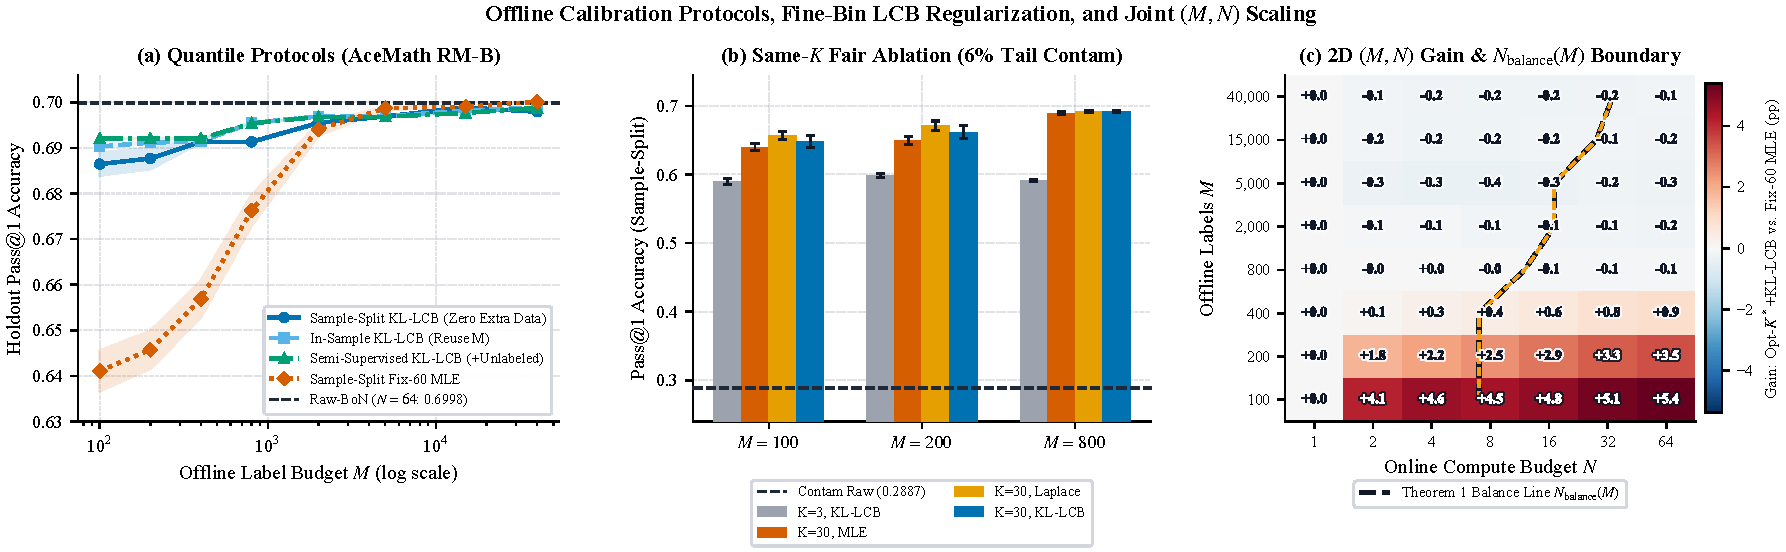
\includegraphics[width=\textwidth]{fig2_joint_mn_and_protocols}
\caption{\textbf{Offline calibration scaling and protocols (\Cref{thm:joint-minimax,prop:spacings}).} \textbf{(a)} Three quantile protocols on \texttt{AceMath RM-B} ($\pm 1$ SE over 50 repeats). \textbf{(b)} Fair same-$K$ calibrator ablation under 6\% tail contamination ($K=3$ vs.\ $K=30$). \textbf{(c)} 2D $(M, N)$ accuracy gain of $N$-agnostic $K^*(M) + \mathrm{KL\text{-}LCB}$ over $\mathrm{Fix\text{-}60\ MLE}$, with the \Cref{thm:joint-minimax} balance boundary $N_{\mathrm{balance}}(M)$.}
\label{fig:joint-mn}
\end{figure}

\Cref{tab:protocols,fig:joint-mn} reveal two findings: (i) \texttt{Sample-Split KL-LCB} sacrifices only $\approx 0.4\,\mathrm{pp}$ at $M=100$ relative to In-Sample/Semi-Supervised (consistent with the factor-2 penalty in \Cref{prop:spacings}) while beating \texttt{Fix-60 MLE} by $+4.53\,\mathrm{pp}$ at $M=100$ and converging for $M \ge 400$ (likewise on \texttt{GPQA-Qwen7B} at $M=5{,}000$: $0.3063 / 0.3065 / 0.3081$ across the three protocols); (ii) at coarse $K=3$, regularizing $K$ drives most gains, whereas isolating a narrow 6\% false-positive tail requires finer bins ($K=30$, gaining $+6.4\text{--}7.4\,\mathrm{pp}$ over $K=3$), where LCB and Laplace outperform same-$K$ MLE by $+1.2\text{--}2.8\,\mathrm{pp}$ at small $M$. On 2D $(M, N)$ surfaces (\Cref{fig:joint-mn}(c)), empirical gains track the balance law~\eqref{eq:n-balance}, while at small-$M$ high-$N$ regimes empirical-Bernstein LCB collapses to $0.6032$ vs.\ $0.6962$ for $\mathrm{KL\text{-}LCB}$ ($M=400, K=20$).

\subsection{Disjoint Holdout Inference and Natural Overoptimization Subsets}

To avoid fold-overlap covariance \citep{nadeau2003inference} and post-selection refit bias, \Cref{tab:single-split} evaluates a disjoint stratified split ($\mathrm{Train}\ 50\% / \mathrm{Val}\ 20\% / \mathrm{Test}\ 30\%$) with frozen predictors ($\mathrm{Hybrid\text{-}Fixed}$, $\varepsilon_{\mathrm{refit}} \equiv 0$, \Cref{alg:hybrid-fixed}) and two-sided paired studentized $t$-tests ($p_t$) across prompts (auxiliary 5-fold permutation checks apply the $+1$ correction of \citet{phipson2010permutation}).

\begin{table}[t]
\centering
\caption{Disjoint single-split ($\mathrm{Train}\ 50\% / \mathrm{Val}\ 20\% / \mathrm{Test}\ 30\%$) primary evaluation across five full benchmarks plus the natural overoptimization subset \texttt{AceMath/college\_math} (\texttt{RM-B}). Bold marks row maximum among fixed candidates; underline on \texttt{college\_math} denotes the branch selected by $\mathrm{Hybrid\text{-}Fixed}$.}
\label{tab:single-split}
\small
\setlength{\tabcolsep}{4.5pt}
\begin{tabular}{lccccccc}
\toprule
Dataset & $P_{\mathrm{test}}$ ($N$) & Selected $\hat{m}$ & $\mathrm{Raw\text{-}BoN}$ & $\mathrm{Pooled\text{-}LCB}$ & $\mathrm{Within\text{-}Z}$ & $\mathrm{Hybrid\text{-}Fixed}$ & $\mathrm{Hybrid} - \mathrm{Pooled}$ ($p_t$) \\
\midrule
\texttt{S3 3-Domain}     & $839$ ($128$)   & $\mathrm{Raw\text{-}BoN}$ & $\mathbf{0.5159}$ & $0.4918$ & $0.5022$ & $\mathbf{0.5159}$ & $+2.41\,\mathrm{pp}$ ($0.0050$) \\
\texttt{RB2 Skywork}     & $556$ ($4$)     & $\mathrm{Raw\text{-}BoN}$ & $\mathbf{0.8592}$ & $0.8409$ & $0.8500$ & $\mathbf{0.8592}$ & $+1.83\,\mathrm{pp}$ ($0.0120$) \\
\texttt{AceMath RM-B}    & $2{,}695$ ($64$)& $\mathrm{Raw\text{-}BoN}$ & $0.7023$ & $\mathbf{0.7050}$ & $0.6733$ & $0.7023$          & $-0.28\,\mathrm{pp}$ ($0.1400$) \\
\texttt{AceMath RM-A}    & $2{,}695$ ($64$)& $\mathrm{Raw\text{-}BoN}$ & $0.7358$ & $\mathbf{0.7365}$ & $0.7074$ & $0.7358$          & $-0.07\,\mathrm{pp}$ ($0.6806$) \\
\texttt{OlympiadBench}   & $202$ ($128$)   & $\mathrm{Raw\text{-}BoN}$ & $0.4010$ & $\mathbf{0.4057}$ & $0.3141$ & $0.4010$          & $-0.47\,\mathrm{pp}$ ($0.6742$) \\
\midrule
\texttt{college\_math RM-B} & $845$ ($64$) & $\mathrm{Pooled\text{-}LCB}$ & $0.4504$ & $0.4559$ & $\mathbf{0.4591}$ & \underline{$0.4559$} & $+0.55\,\mathrm{pp}$ vs.\ $\mathrm{Raw}$ ($0.1810$)$^*$ \\
\bottomrule
\end{tabular}
\vspace{2pt}
{\footnotesize $^*$On the full \texttt{college\_math RM-B} cohort ($P=2{,}818$), $\mathrm{Raw\text{-}BoN}$ peaks at $N=16$ ($0.4640$) and drops to $0.4579$ at $N=64$ ($-0.60 \pm 0.26\,\mathrm{pp}$, $p_t = 0.0208$); on the smaller 30\% split ($P_{\mathrm{test}}=845$), $\mathrm{Hybrid\text{-}Fixed}$ selects $\mathrm{Pooled\text{-}KL\text{-}LCB}$ over $\mathrm{Raw\text{-}BoN}$ ($+0.55\,\mathrm{pp}$, $p_t = 0.1810$).}
\end{table}

On the five uncontaminated benchmarks (\Cref{tab:single-split}, \Cref{fig:simpson}(a)), $\mathrm{Hybrid\text{-}Fixed}$ selects $\mathrm{Raw\text{-}BoN}$, avoiding $\mathrm{Pooled\text{-}KL\text{-}LCB}$'s cross-domain Simpson confounding on \texttt{S3} ($+2.41\,\mathrm{pp}, p_t=0.0050$) and \texttt{RB2} ($+1.83\,\mathrm{pp}, p_t=0.0120$), while avoiding $\mathrm{Within\text{-}Prompt\text{-}Z}$'s ceiling losses on low-shift math pools ($-2.91$ to $-9.16\,\mathrm{pp}$ vs.\ $\mathrm{Pooled}$, \Cref{thm:sample-z-ceiling}; empirical refit shift $\hat{\varepsilon}_{\mathrm{refit}} \in [0.0006, 0.0074]$). Across all subsets, \texttt{AceMath/college\_math} (\texttt{RM-B}, $P=2{,}818$, zero synthetic modification) exhibits statistically significant natural overoptimization (\Cref{fig:simpson}(b)): $\mathrm{Raw\text{-}BoN}$ drops from $0.4640$ ($N=16$) to $0.4579$ ($N=64$, $-0.60 \pm 0.26\,\mathrm{pp}, p_t = 0.0208$), and $\mathrm{Hybrid\text{-}Fixed}$ switches to $\mathrm{Pooled\text{-}KL\text{-}LCB}$ ($0.4559$ vs.\ $0.4504$, $p_t=0.1810$; $\mathrm{Within\text{-}Z}$ attains $0.4591$).

\begin{figure}[t]
\centering
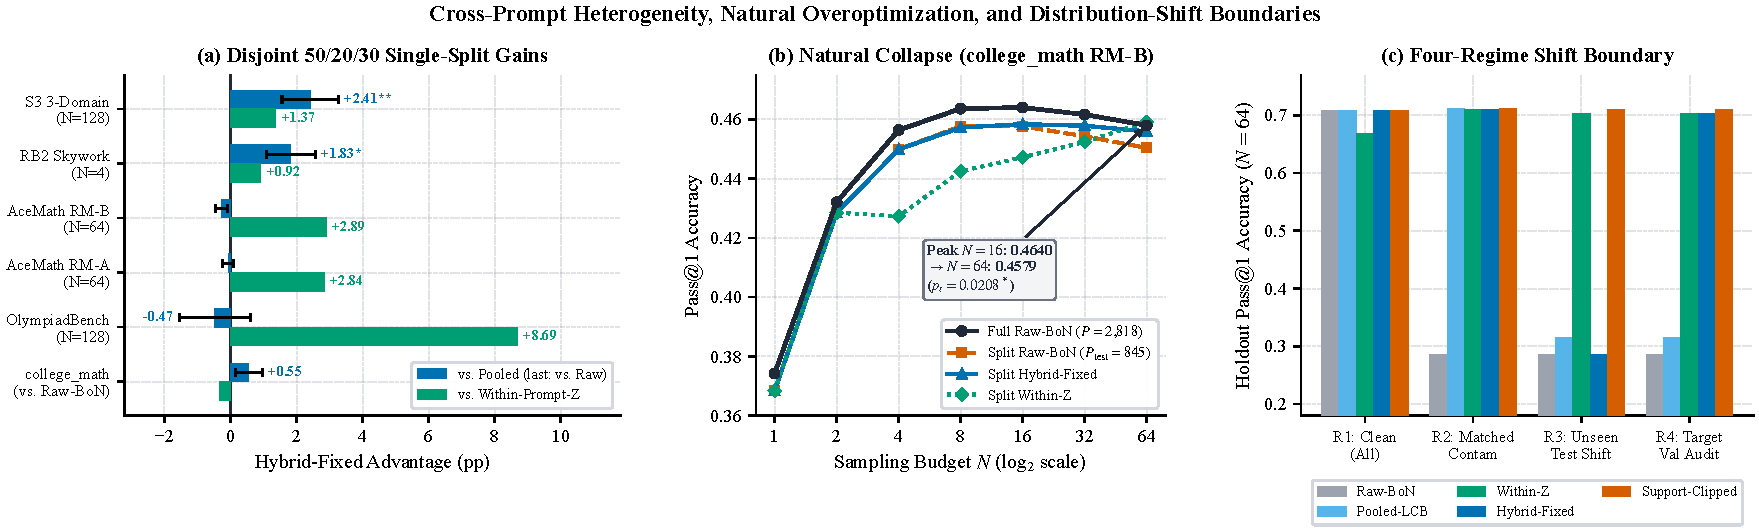
\includegraphics[width=\textwidth]{fig3_heterogeneity_and_shift}
\caption{\textbf{Cross-prompt heterogeneity and distribution shift (\Cref{sec:heterogeneity}).} \textbf{(a)} Paired Pass@1 gains of $\mathrm{Hybrid\text{-}Fixed}$ on disjoint 50/20/30 test splits ($^{**}\,p_t < 0.01$, $^{*}\,p_t < 0.05$). \textbf{(b)} Natural overoptimization curve on uncontaminated \texttt{AceMath/college\_math RM-B}. \textbf{(c)} Four-regime shift matrix on \texttt{AceMath RM-B} ($N=64$).}
\label{fig:simpson}
\end{figure}

\subsection{Controlled Score-Tail Contamination and Distribution Shift}

We inject false-positive spikes ($> q_{0.995} + 0.8\sigma$) into $6\%$ of wrong trajectories on \texttt{AceMath RM-B} ($P_{\mathrm{test}}=2{,}695, N=64$) across four train/val/test shift regimes (\Cref{tab:shift,fig:simpson}(c)), alongside $\mathrm{Support\text{-}Clipped\text{-}KL\text{-}LCB}$ (\Cref{alg:split-kl-lcb} with $\tau_{\mathrm{clip}} = 0.998$).

\begin{table}[t]
\centering
\caption{Four-regime distribution-shift matrix under controlled $6\%$ wrong-tail spike contamination on \texttt{AceMath RM-B} ($N=64, P_{\mathrm{test}}=2{,}695$; bold marks row maximum, underline marks $\mathrm{Hybrid\text{-}Fixed}$ selection).}
\label{tab:shift}
\small
\begin{tabular}{llccccc}
\toprule
Train / Val $\to$ Test Regime & Val Selected $\hat{m}$ & $\mathrm{Raw\text{-}BoN}$ & $\mathrm{Pooled\text{-}LCB}$ & $\mathrm{Within\text{-}Z}$ & $\mathrm{Hybrid\text{-}Fixed}$ & $\mathrm{Support\text{-}Clipped}$ \\
\midrule
1. Clean / Clean $\to$ Clean         & $\mathrm{Raw\text{-}BoN}$ & $0.7083$ & $\mathbf{0.7090}$ & $0.6690$ & \underline{$0.7083$} & $\mathbf{0.7090}$ \\
2. Contam / Contam $\to$ Contam      & $\mathrm{Within\text{-}Z}$& $0.2865$ & $\mathbf{0.7124}$ & $0.7093$ & \underline{$0.7093$} & $\mathbf{0.7124}$ \\
3. Clean / Clean $\to$ Contam (Unseen)& $\mathrm{Raw\text{-}BoN}$& $0.2865$ & $0.3159$ & $0.7024$ & \underline{$0.2865$} & $\mathbf{0.7108}$ \\
4. Clean / Contam $\to$ Contam       & $\mathrm{Within\text{-}Z}$& $0.2865$ & $0.3159$ & $0.7024$ & \underline{$0.7024$} & $\mathbf{0.7108}$ \\
\bottomrule
\end{tabular}
\end{table}

Under matched contamination (Regime~2), $\mathrm{Hybrid\text{-}Fixed}$ prevents collapse ($0.7093$ vs.\ $0.2865$, $+42.29\,\mathrm{pp}, p_t < 10^{-300}$). Under completely unseen test shift (Regime~3), clean-trained $\mathrm{Pooled\text{-}KL\text{-}LCB}$ also drops to $0.3159$ because out-of-support spikes land in its open top bin $(\hat{e}_{K-1}, +\infty)$; by contrast, $\mathrm{Within\text{-}Prompt\text{-}Z}$ retains $0.7024$ because zero-success prompts down-weight its extreme Z-tail (\Cref{thm:sample-z-ceiling}(1)). Thus either target validation auditing (Regime~4: $0.7024$) or upper support clipping ($0.7108$) restores safety.

\subsection{Multi-Verifier Correlation Structure on RewardBench-2 and OlympiadBench}

\Cref{fig:multi-rm} evaluates \Cref{sec:ensemble} on real multi-RM benchmarks. Across RM families (\Cref{fig:multi-rm}(a)), homogeneous AllenAI models exhibit severe shared wrong-answer correlation ($\bar{\rho}_0 = 0.9088$, Copula $\eta_0 = 0.9284$ on \texttt{RB2 Homo-4}), whereas cross-family RMs decouple wrong answers ($\bar{\rho}_0 = 0.6359, \eta_0 = 0.6437$ on \texttt{RB2 Hetero-6}; $\bar{\rho}_0 = 0.2221$ across \texttt{uPRM-70B+32B}). On \texttt{RB2 Hetero-6} ($P=1{,}723, N=4$, 5-fold CV, \Cref{fig:multi-rm}(b)), $\mathrm{Fisher}(\tau=-1)$ achieves $0.8828$ and $\mathrm{Bayes\ QDA}$ achieves $0.8793$, while enforcing the conservative $\kappa \le 1$ tail constraint targets $N=2$ SNR trade-offs ($\mathrm{Safe\text{-}Fisher}=0.8166$; unconstrained $\mathrm{GenEig}=0.3929$ confirms \Cref{thm:gaussian-ensemble}(1)). On \texttt{OlympiadBench} ($P=674, N=1\dots 128$, \Cref{fig:multi-rm}(c)), calibrated weighted $\mathrm{BoN}$ on 70B reaches $0.4733$ and cross-view $\mathrm{Logit\text{-}Stack}$ reaches $0.4436$ at $N=128$, outperforming single \texttt{uPRM-70B} ($0.4154$) and \texttt{uPRM-32B} ($0.3694$). Separately, a $3\times 3$ degenerate zero-KKT matrix ($|I_+|=2, I_0=\{3\}$) matches the corrected asymptotic $\frac{1}{4\pi}t^{-2}e^{-t^2}$ at $t=500$ with numerical ratio $1.0022$ (\Cref{thm:gaussian-ensemble}(2)).

\begin{figure}[t]
\centering
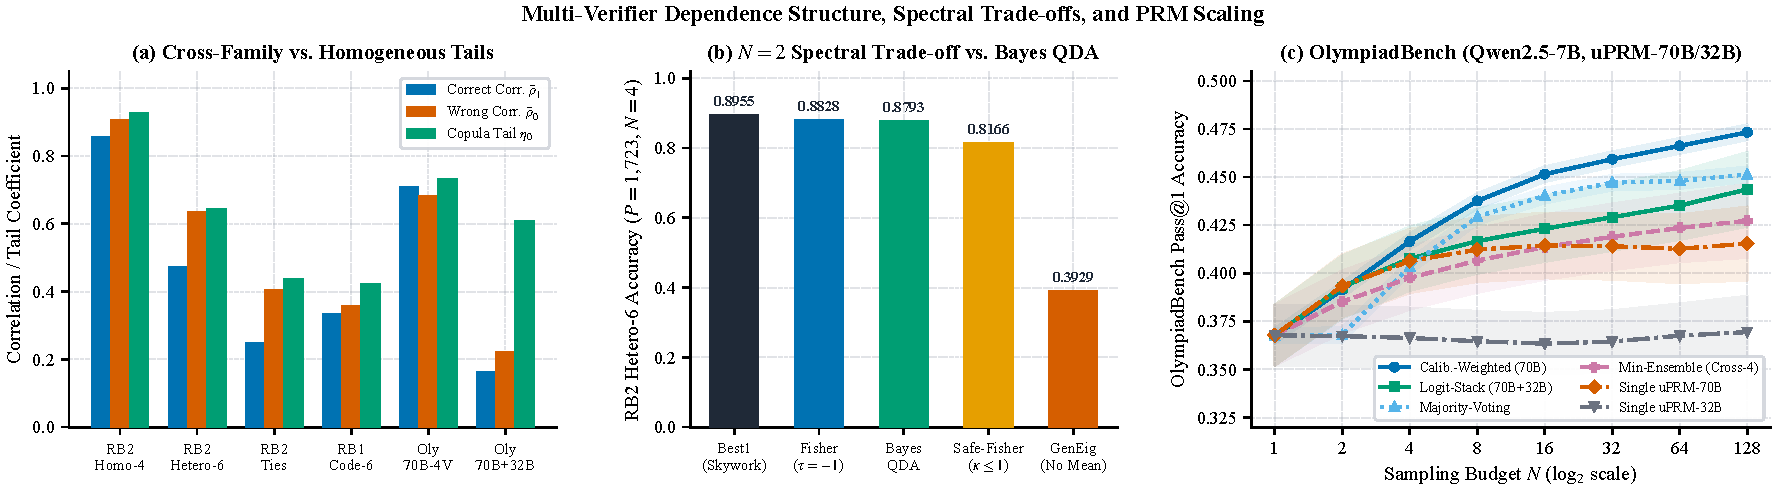
\includegraphics[width=\textwidth]{fig4_multi_rm_dependence}
\caption{\textbf{Multi-verifier dependence and PRM scaling (\Cref{sec:ensemble}).} \textbf{(a)} Cross-family vs.\ homogeneous conditional correlations $(\bar{\rho}_1, \bar{\rho}_0)$ and Copula tail coefficient $\eta_0$. \textbf{(b)} \texttt{RB2 Hetero-6} spectral path comparison ($P=1{,}723, N=4$). \textbf{(c)} \texttt{OlympiadBench} (\texttt{Qwen2.5-7B}, \texttt{uPRM-70B/32B}) Pass@1 scaling up to $N=128$.}
\label{fig:multi-rm}
\end{figure}

\section{Discussion, Limitations, and Broader Impact}
\label{sec:discussion}

\paragraph{Practical Takeaways.}
Empirical verification and minimax bounds support a conservative calibration strategy: passive calibration should not override an already monotone verifier on clean heterogeneous workloads; scaling compute beyond $N_{\mathrm{balance}}(M)$ requires scaling calibration labels $M$; within-prompt Z-scores exchange raw shift invariance for an asymptotic ceiling loss whenever $\pi_0 > 0$; and holdout gating should be paired with support clipping when test-time score shifts are unforeseen.

\paragraph{Limitations.}
Our theoretical guarantees carry four explicit scope limits: (1) our joint minimax theorems assume one-dimensional continuous marginal scores $S \in \R$ on a fixed prompt distribution, leaving discrete ties handled empirically via uniform randomization; (2) passive calibration requires historical coverage of the tail regime and cannot detect novel out-of-support reward hacking unless target validation labels or upper quantile clipping (\Cref{alg:split-kl-lcb}) are available; (3) the three-branch gate assumes candidate responses across prompts can be partitioned at the prompt level without dynamic adaptive sampling per question; and (4) the multi-verifier Gaussian and Copula tail laws provide exact parametric insight rather than distribution-free finite-sample bounds under heavy-tailed dependence.

\paragraph{Broader Impact and Reproducibility Statement.}
Clarifying when inference scaling saturates or collapses prevents silent reasoning failures and wasted test-time GPU compute in safety-critical coding and mathematical assistants, while exposing vulnerabilities to adversarial high-score wrong outputs. All theory scripts, 73 offline unit tests, and benchmark evaluation pipelines use deterministic random seeds without external proprietary API dependencies and are indexed in \Cref{app:index} (\Cref{tab:index}); compliance details follow in \Cref{app:checklist}.

\bibliographystyle{plainnat}
\bibliography{references}

\newpage
\appendix
\counterwithin{theorem}{section}
\counterwithin{proposition}{section}

\section{Single-Verifier Preliminaries (Repo Theorems 1--4)}
\label{app:preliminaries}

For completeness, we summarize and prove the single-verifier preliminary statements used in \Cref{sec:model} (preserving repository numbering in parentheses).

\begin{theorem}[Exact Order-Statistic Integral with Tie Atoms; Repo Theorem 1]
\label{thm:app-pit}
Let $F_1, F_0$ be arbitrary CDFs on $\R$ with countable atom set $\mathcal{A}$, mixture $\Fmix = p F_1 + (1-p)F_0$, and uniform random tie-breaking on $\mathcal{I}_{\max}$. Then~\eqref{eq:pit-exact} holds for all $N \ge 1$, with $q(a) = \frac{p\Delta F_1(a)}{\Delta\Fmix(a)}$ at $a \in \mathcal{A}$. For Gaussian $S \mid Y=c \sim \mathcal{N}(\mu_c, \sigma_c^2)$, $P_{\mathrm{BoN}}(2) - p = p(1-p)[2\Phi(\frac{\mu_1-\mu_0}{\sqrt{\sigma_1^2+\sigma_0^2}}) - 1]$ and $P_{\mathrm{Anti\text{-}BoN}}(2) = 2p - P_{\mathrm{BoN}}(2)$.
\end{theorem}
\begin{proof}
At any atom $a \in \mathcal{A}$, conditional correctness of a uniformly chosen tied maximizer equals $q(a)$, while $\Prob(S_{(N)} = a) = [\Fmix(a)]^N - [\Fmix(a-)]^N = \Delta([\Fmix]^N)(a)$. Pushforward equivalence with $v \mapsto \Fmix^{-1}(v^{1/N})$ follows from the Galois connection $\Fmix^{-1}(u) \le x \iff u \le \Fmix(x)$.
\end{proof}

\begin{theorem}[Heavy Wrong-Tail Collapse, $C^1/C^0$ MLRP, and Fixed-Peak Gumbel Constant; Repo Theorem 2]
\label{thm:app-collapse}
Let $F_1, F_0$ have positive densities $f_1, f_0$ on an open interval $I$ with right endpoint $x_R$.
\begin{enumerate}[leftmargin=1.8em,itemsep=2pt]
    \item If $\lim_{x\uparrow x_R} f_1(x)/f_0(x) = 0$, then $\lim_{N\to\infty} P_{\mathrm{BoN}}(N) = 0$ and $\arg\max_{N\ge 1} P_{\mathrm{BoN}}(N)$ is finite.
    \item Under $f_1, f_0 \in C^1(I)$ (over closed subintervals $[a,b] \subset I$) or $f_1, f_0 \in C^0(I)$ (over unions of two disjoint closed intervals $I_1 \cup I_2 \subset I$), $P_{\mathrm{BoN}}(N+1; A) \ge P_{\mathrm{BoN}}(N; A)$ holds for all $p \in (0, 1), N \ge 1$ iff $\Lambda(x) = f_1(x)/f_0(x)$ is non-decreasing on $I$. For Gaussians with $\kappa = \sigma_0/\sigma_1 < 1$ and $\Delta\mu = 0$, $P_{\mathrm{BoN}}(1) = P_{\mathrm{BoN}}(2) = p$ followed by strict increase $P_{\mathrm{BoN}}(N) \uparrow 1$ for $N \ge 2$.
    \item \textbf{(Fixed-Peak-Height Gumbel Limit)} For Gaussian $\sigma_0 = \kappa\sigma_1$ ($\kappa > 1$) under $\Delta\mu(\kappa) := \sigma_1\sqrt{c_1(\kappa^2-1)}$ ($c_1 > 0$), let $x_{\mathrm{peak}} = \frac{\mu_1\sigma_0^2 - \mu_0\sigma_1^2}{\sigma_0^2 - \sigma_1^2}$, $\tau^{-2} = \sigma_1^{-2} - \sigma_0^{-2}$, $N_0^* = 1/\barFmix(x_{\mathrm{peak}})$, and $h = \fmix(x_{\mathrm{peak}})/\barFmix(x_{\mathrm{peak}})$. As $\kappa \downarrow 1^+$, $q_{\mathrm{peak}}(\kappa) \to \sigma(\logit(p) + c_1/2) \in (0, 1)$, $h(\kappa)\tau(\kappa) \sim \frac{\sqrt{c_1}}{\kappa^2 - 1} \to +\infty$, and $\frac{2(h\tau)^2}{q_{\mathrm{peak}}(1-q_{\mathrm{peak}})}(q_{\mathrm{peak}} - \E[q(S_{(e^\delta N_0^*)})]) \to (\delta + \gamma)^2 + \frac{\pi^2}{6}$ uniformly on $[-D, D]$, yielding $\lim_{\kappa \downarrow 1^+} N^*_{\mathrm{exact}} / N_0^* = e^{-\gamma} \approx 0.561459$.
\end{enumerate}
\end{theorem}
\begin{proof}
Parts (1)--(2) follow from Stieltjes integration by parts $P_{\mathrm{BoN}}(N+1)-P_{\mathrm{BoN}}(N) = \int \Fmix^N(1-\Fmix)\,dq$ and the two-interval identity $P_{\mathrm{BoN}}(2; I_1\cup I_2) - P_{\mathrm{BoN}}(1; I_1\cup I_2) \to -w_1^* w_2^*(q(x_1)-q(x_2)) < 0$ when $q(x_1) > q(x_2)$ ($x_1 < x_2$). For (3), setting $\mu_0 = 0$ gives $x_{\mathrm{peak}} = \frac{\kappa^2\sigma_1\sqrt{c_1}}{\sqrt{\kappa^2-1}}$, $h \sim \frac{\sqrt{c_1}}{\sigma_1\sqrt{\kappa^2-1}}$, and $\tau = \frac{\kappa\sigma_1}{\sqrt{\kappa^2-1}}$. Writing $q(x_{\mathrm{peak}}+y) = g(y^2/(2\tau^2))$ with $g(u) = \sigma(L_0 - u)$ bounds the fourth-order Taylor remainder on $|y| \le \sqrt{2}\tau$. The normalized maximum $G_N = h(S_{(N_\delta)} - x_{\mathrm{peak}}) - \delta$ converges in distribution and fourth moments to $\mathrm{Gumbel}(0,1)$ via monotone normal hazard bounds and left-tail truncation at $a := \frac{1}{2}x_{\mathrm{peak}}$; Karlin single-crossing unimodality locks $N^*_{\mathrm{exact}}/N_0^* \to e^{-\gamma}$.
\end{proof}

\begin{theorem}[Binary Verifier Scaling and Calibrated Weighted Majority; Repo Theorems 3 \& 4]
\label{thm:app-cal}
(i) For binary $S_i \in \{0,1\}$ with $\alpha = \mathrm{TPR} > \beta_{\mathrm{fp}} = \mathrm{FPR}$, $q_1 = p\alpha + (1-p)\beta_{\mathrm{fp}}$, and $\mathrm{PPV} = p\alpha/q_1$, $P_{\mathrm{BoN,bin}}(N) = \mathrm{PPV} - C(1-q_1)^N$ with $C = \frac{p(1-p)(\alpha-\beta_{\mathrm{fp}})}{q_1(1-q_1)}$; when $\beta_{\mathrm{fp}} = 0$ ($\mathrm{PPV}=1$), $\DKL(P_N \| \delta_1) = +\infty$ while $\TV(P_N, \delta_1) = \frac{1-p}{1-p\alpha}(1-p\alpha)^N$ and $\DKL(\delta_1 \| P_N) = \Theta((1-p\alpha)^N)$. (ii) Over countably infinite wrong answers $\{a_j\}_{j\ge 1}$ with weights $W_i \in [0, w_{\max}]$, if $\Delta_{\min} := p\mu_{w,+} - \sup_j(p_j\mu_{w,j}) > 0$, grouping the tail $\sum_{j>K_0}p_j < \frac{p\mu_{w,+}}{2w_{\max}}$ into a super-bucket yields $\Prob(\hat{A}_N \neq a^*) \le (K_0+1)e^{-c N}$.
\end{theorem}

\section{Proofs for Section~\ref{sec:minimax} (Joint Minimax and Spacings)}
\label{app:minimax}

\begin{proof}[Proof of \Cref{thm:joint-minimax}]
\textbf{Part 1:} On $\mathcal{F}_\beta^{\mathrm{sep}}$, for $\varepsilon \in (0, \varepsilon_\eta)$, $\{x : q(x) > q^* - \varepsilon\} \subset U_\eta$ gives $\bar{F}_Q(q^* - \varepsilon) = (1+o(1))\frac{2f^*}{C^{1/\beta}}\varepsilon^{1/\beta}$; substituting $u = N^\beta\varepsilon$ and dominated convergence yield $\frac{\Gamma(\beta+1)C}{(2f^*)^\beta}N^{-\beta}$.

\textbf{Part 2:} For $K > \frac{2}{\eta_0 f_{\min}}$, any equal-frequency bin inside $U_{\eta_0}$ has width $\le \frac{1}{K f_{\min}} < \frac{\eta_0}{2}$. Let $i^{\mathrm{near}} = \arg\min_{1\le i\le N}|S_i - x^*|$, $D_N = |S_{i^{\mathrm{near}}} - x^*|$, $k^{\mathrm{near}} = k(S_{i^{\mathrm{near}}})$, and $\hat{k}^* = k(S_{\hat{i}^*})$. Conditioning on $\mathcal{F}_{\mathrm{bins}} = \sigma(\mathcal{D}_M, k(S_1),\dots,k(S_N))$ gives $\E[Y_{\hat{i}^*} \mid \mathcal{F}_{\mathrm{bins}}] = q_{\hat{k}^*}$. Define three offline bad events, each of probability $\le \frac{1}{3M}$: $\mathcal{B}_1 = \{\exists k: \hat{s}_k^{\mathrm{KL\text{-}LCB}}(\frac{1}{3M}) > q_k\}$ (Cram\'er--Chernoff + union bound), $\mathcal{B}_2 = \{\exists k: m_k < \frac{M}{2K}\}$ (multiplicative Chernoff for $M \ge 8K\ln(3KM)$), and $\mathcal{B}_3 = \{\exists k: m_k \ge 1,\ q_k - \hat{q}_k > \sqrt{\frac{\ln(3KM)}{2m_k}}\}$ (conditional Hoeffding). Let $\mathcal{B}_{\mathrm{miss}} = \{D_N > \eta_0/2\}$, which has probability $\le (1 - \eta_0 f_{\min})^N \le e^{-\eta_0 f_{\min}N}$. On $\mathcal{G} = (\mathcal{B}_1 \cup \mathcal{B}_2 \cup \mathcal{B}_3 \cup \mathcal{B}_{\mathrm{miss}})^c$, $B_{k^{\mathrm{near}}} \subset U_{\eta_0}$ and $(a+b)^\beta \le c_\beta(a^\beta + b^\beta)$ yield $q^* - q_{k^{\mathrm{near}}} \le C_1 c_\beta D_N^\beta + \frac{C_1 c_\beta}{(K f_{\min})^\beta}$. By $\mathcal{B}_1^c, \mathcal{B}_2^c, \mathcal{B}_3^c$ and Pinsker's inequality $\KL(\hat{q}_k, \hat{s}_k^{\mathrm{KL\text{-}LCB}}) \ge 2(\hat{q}_k - \hat{s}_k^{\mathrm{KL\text{-}LCB}})^2$,
\[
q_{\hat{k}^*} \ge \hat{s}_{\hat{k}^*}^{\mathrm{KL\text{-}LCB}} \ge \hat{s}_{k^{\mathrm{near}}}^{\mathrm{KL\text{-}LCB}} \ge q_{k^{\mathrm{near}}} - 2\sqrt{\frac{\ln(3KM)}{2m_{k^{\mathrm{near}}}}} \ge q_{k^{\mathrm{near}}} - 2\sqrt{\frac{K\ln(3KM)}{M}}.
\]
Integrating $\E[\ind_{\mathcal{G}}D_N^\beta] \le \int_0^{\eta_0/2}\beta r^{\beta-1}e^{-2f_{\min}Nr}\,dr \le \frac{\Gamma(\beta+1)}{(2f_{\min})^\beta}N^{-\beta}$ yields~\eqref{eq:joint-upper}.

\textbf{Part 3:} Construct $J = \Theta(h^{-1})$ disjoint bumps $q_j(x) = \frac{1}{2} + c_\beta h^\beta\max(0, 1 - |x-t_j|^\beta/h^\beta)$ on $[0.2, 0.8]$ with $\fmix \equiv 1$ ($c_\beta \le C_1$). Because unlabeled $S_{1:N} \sim \mathrm{Unif}(0,1)^N$ carry zero information about $j$, $\DKL(P_j^{\otimes M}\otimes\mathrm{Unif}^N \| P_0^{\otimes M}\otimes\mathrm{Unif}^N) = M\DKL(P_j\|P_0) \le C_2 M h^{2\beta+1}$. Choosing $h \asymp (\frac{\ln M}{M})^{\frac{1}{2\beta+1}}$ and Fano's inequality gives $\Omega((\frac{\ln M}{M})^{\frac{\beta}{2\beta+1}})$; evaluating at $P^*$ gives $\Omega(N^{-\beta})$ by Part~1.
\end{proof}

\begin{proof}[Proof of \Cref{prop:spacings}]
By continuity of $\Fmix$ and Pyke's representation \citep{pyke1965spacings}, $(\hat{\pi}_1,\dots,\hat{\pi}_K) \stackrel{d}{=} (G_1/G_{\mathrm{tot}},\dots,G_K/G_{\mathrm{tot}})$ where $G_k \sim \mathrm{Gamma}(d_k, 1)$ and $G_{\mathrm{tot}} \sim \mathrm{Gamma}(M_1+1, 1)$ with $\frac{11}{12}\frac{M_1+1}{K} \le d_k \le \frac{13}{12}\frac{M_1+1}{K}$ when $M_1+1 \ge 12K$. For $\psi(c) = c - 1 - \ln c$, $\min(\psi(0.60), \psi(1.65)) \approx 0.11082 > \frac{1}{9.1}$ and $\min(\psi(0.90), \psi(1.10)) \approx 0.0046898 > \frac{1}{214}$. Thus $d_{\min} \ge 9.1\ln(16KM)$ and $M_1+1 \ge 214\ln(16M)$ ensure $G_k \in [0.60 d_k, 1.65 d_k]$ ($\forall k$) and $G_{\mathrm{tot}} \in [0.90(M_1+1), 1.10(M_1+1)]$ w.p.\ $\ge 1 - \frac{1}{4M}$, giving $\frac{0.60\times 11/12}{1.10 K} = \frac{1}{2K} \le \hat{\pi}_k \le \frac{1.65\times 13/12}{0.90 K} = \frac{143}{72K} < \frac{2}{K}$. Conditioning on $\mathcal{D}_{M_1}^{\mathrm{edge}}$, $M_2 \ge 16K\ln(4KM)$ yields $\Prob(\exists k: m_k < \frac{M_2}{4K} \mid \mathcal{D}_{M_1}^{\mathrm{edge}}) \le \frac{1}{4M}$. Substituting $m_k \ge \frac{M_2}{4K} \ge \frac{M}{8K}$ into $\sqrt{\frac{2\ln(4KM)}{m_k}} \le 4\sqrt{\frac{K\ln(4KM)}{M}}$ completes the proof.
\end{proof}

\section{Proofs for Section~\ref{sec:heterogeneity} (Prompt Heterogeneity and Sample-$Z_{i,N}$)}
\label{app:heterogeneity}

\begin{proof}[Proof of \Cref{thm:simpson}]
Differentiating $w(x\mid s) = f_{\mathrm{mix},x}(s)/f_{\mathrm{pool}}(s)$ gives $\partial_s w(x\mid s) = w(x\mid s)(g_x(s) - \E[g_X(s)\mid S=s])$, establishing (1). For (2), on $s \in [3.5, 4.2]$:
\begin{enumerate}[leftmargin=1.8em,itemsep=2pt]
    \item $\ell'_1(s) = -0.75(s - 0.4) \in [-2.85, -2.325] < 0$ and $\ell'_2(s) = -0.75(s - 3.4) \in [-0.60, -0.075] < 0$. Hence $q_1, q_2$ decrease strictly on $[3.5, 4.2]$, locking $q_1(s) \in [4.750\times 10^{-4},\, 2.900\times 10^{-3}]$ and $q_2(s) \in [0.96810,\, 0.97464]$, so $q_2(s) - q_1(s) > 0.96519$. Since $u \mapsto u(1-u)$ decreases strictly on $(0.5, 1)$, $\partial_s q_2(s) \le -0.075\, q_2(3.5)(1-q_2(3.5)) \approx -1.8539\times 10^{-3} < -1.85\times 10^{-3}$ and $|\partial_s q_2(s)| \le 0.60\, q_2(4.2)(1-q_2(4.2)) < 0.01915$, while $\partial_s q_1(s) < -1.10\times 10^{-3}$ and $|\partial_s q_1(s)| < 0.00827$, giving $|\E[\partial_s q_X(s)\mid S=s]| < 0.01915$.
    \item All four Gaussian means $\{0.3, 0.0, 3.3, 3.0\} < 3.5$, so $r(s) = \frac{0.15 f_{\mathrm{mix},2}(s)}{0.85 f_{\mathrm{mix},1}(s)} \in [1.1211, 3.2180]$ and $w_1(s)w_2(s) = \frac{r(s)}{(1+r(s))^2} \ge \frac{3.2180}{4.2180^2} > 0.18087$.
    \item Component convex combinations give $g_1(s) \le -0.25 s$ and $g_2(s) \ge -(s - 3.3)$, so $g_2(s) - g_1(s) \ge 3.3 - 0.75 s \ge 3.3 - 0.75\times 4.2 = +0.15$.
\end{enumerate}
Multiplying yields $\Cov(Y, g_X(s)\mid S=s) > 0.18087\times 0.96519\times 0.15 > 0.02618$, so $q'_{\mathrm{pool}}(s) > 0.02618 - 0.01915 = +7.03\times 10^{-3}$ (more precisely $+7.044\times 10^{-3}$) $> 0$ for all $s \in [3.5, 4.2]$.
\end{proof}

\begin{proof}[Proof of \Cref{thm:zscore-n2,thm:sample-z-ceiling,prop:hybrid}]
In \Cref{thm:zscore-n2}(2), exchangeability gives $P_{\mathrm{Cal\text{-}BoN}}^{\mathrm{oracle}}(2) - P_{\mathrm{Raw}}(2) = 2\E[(q_X(S_1)-q_X(S_2))\ind\{S_1<S_2, q_X(S_1)>q_X(S_2)\}]$ and symmetrically for $\mathrm{Anti\text{-}BoN}(2)$, establishing the bidirectional equivalence. In \Cref{thm:sample-z-ceiling}(1), boundary strata ($p \in \{0,1\}$) have $Z^* \sim \mathcal{N}(0,1)$ whereas interior strata have variance $v(p) \le v_{\max} < 1$, decaying as $o(\phi(z))$ as $z \to +\infty$. For (2), $Z_{i,N} = (\tilde{S}_i - \bar{\tilde{S}}_N)/\hat{\tilde{s}}_N$ is $(b(X), a(X))$-invariant. At fixed $X=x$, sub-Gaussianity gives $\max_{1\le i\le N}|Z_i^*(x)| = O_p(\sqrt{\ln N})$, $|\bar{\tilde{S}}_N - \tilde{\mu}(x)| = O_p(N^{-1/2})$, and $|\hat{\tilde{s}}_N - \tilde{\sigma}(x)| = O_p(N^{-1/2})$, hence $\Delta_N(x) = O_p(\sqrt{(\ln N)/N}) \xrightarrow{p} 0$. Since $q_{\mathrm{pool}, Z^*}$ vanishes at $\pm\infty$, $\operatorname{dist}(Z_{\hat{i}_N}^*(x), K^*) \xrightarrow{p} 0$; bounded convergence on $q_x(b(x)+a(x)[\tilde{\mu}(x)+\tilde{\sigma}(x)Z_{\hat{i}_N}^*(x)]) \equiv \tilde{q}_x(\tilde{\mu}(x)+\tilde{\sigma}(x)Z_{\hat{i}_N}^*(x))$ yields the strict limit $< 1-\pi_0$. \Cref{prop:hybrid} follows from Hoeffding's inequality over $2|\mathcal{M}|$ events and the triangle inequality.
\end{proof}

\section{Proofs for Section~\ref{sec:ensemble} (Multi-Verifier Ensembles)}
\label{app:ensemble}

\begin{proof}[Proof Sketch of \Cref{thm:gaussian-ensemble,thm:copula}]
Simultaneous congruence $P^\top\Sigma_1 P = I_K, P^\top\Sigma_0 P = \operatorname{diag}(\lambda_1,\dots,\lambda_K)$ with $x_k = v_k^2 \ge 0$ converts the constrained $N=2$ $\SNR_2^2$ problem into maximizing the concave objective $\sum_k |d_k|\sqrt{x_k}$ over two linear constraints; Slater strong duality yields $\mathbf{w}_\tau = (\Sigma_0 - \tau\Sigma_1)^{-1}\Delta\boldsymbol{\mu}$ with $R'(\tau) < 0$ by Cauchy--Schwarz. For $M_{\min}(\mathbf{S})$, differentiating $\Prob(M_{\min} > t \mid Y=c)$ across $K$ orthant faces and invoking the KKT identity $\Sigma_{c, I_{0,c}I_{+,c}}\Sigma_{c, I_{+,c}I_{+,c}}^{-1}\mathbf{1}_{I_{+,c}} = \mathbf{1}_{I_{0,c}}$ cancels the linear $t\mathbf{1}_{I_{0,c}}$ term on weakly active coordinates $I_{0,c}$, yielding Schur-complement constant $\alpha_{c, I_0}$ on $k \in I_{+,c}$ while faces $k \in I_{0,c}$ contribute $O(t^{-1})$ lower order. Substituting $h_c(t) = \sqrt{2\alpha_c\ln t}(1+o(1))$ gives $(\ln t)^{(\gamma_c - |I_{+,c}|)/2}$; $2\times 2$ Schur positivity gives $\gamma_c(R_c) > 1$ for $K \ge 2$, and Slepian's lemma gives $\eta_c \ge 1/K$ under $(R_c)_{ij} \ge 0$.
\end{proof}

\section{Reproducibility Index and Benchmark Summary}
\label{app:index}

\begin{table}[h]
\centering
\caption{Traceability mapping across paper claims, proof documents, and repository Python implementations, together with benchmark scale parameters.}
\label{tab:index}
\small
\begin{tabular}{lll}
\toprule
Paper Result & \texttt{PROOF.md} Section & Python Module \& Core Function \\
\midrule
\Cref{thm:joint-minimax} & \S 2.1--2.3 (Theorems 6A--6C) & \texttt{calibration\_theory.py}: \texttt{tight\_joint\_minimax\_scaling} \\
\Cref{prop:spacings}     & \S 2.4 (Proposition 6.1)      & \texttt{calibration\_theory.py}: \texttt{empirical\_quantile\_spacings\_bounds} \\
\Cref{thm:simpson}       & \S 3.1 (Theorem 7A)           & \texttt{heterogeneity\_theory.py}: \texttt{diagnose\_simpson\_confounding} \\
\Cref{thm:zscore-n2}     & \S 3.2 (Theorem 7B)           & \texttt{heterogeneity\_theory.py}: \texttt{diagnose\_within\_prompt\_residual} \\
\Cref{thm:sample-z-ceiling} & \S 3.3 (Theorem 7C)        & \texttt{heterogeneity\_theory.py}: \texttt{verify\_sample\_zscore\_extremal\_convergence} \\
\Cref{prop:hybrid}       & \S 3.4 (Proposition 7.1)      & \texttt{real\_eval.py}: \texttt{evaluate\_single\_split\_prompt\_heterogeneity} \\
\Cref{thm:gaussian-ensemble,thm:copula} & \S 4.1--4.2 (Theorem 5) & \texttt{ensemble\_theory.py}: \texttt{solve\_positive\_quadrant\_qp} \\
\Cref{thm:app-pit,thm:app-collapse,thm:app-cal} & Appendix A (Theorems 1--4) & \texttt{theorems.py}, \texttt{integrals.py}, \texttt{algorithms.py} \\
\bottomrule
\end{tabular}
\end{table}

All experiments fix random seeds across 50 calibration repeats and 50/20/30 stratified splits: \texttt{RB2} ($P=1{,}855, N=4$), \texttt{RB1} ($P=2{,}985$), \texttt{OlympiadBench} ($P=674, N=128$), \texttt{Strategic-TTC} ($P=2{,}798, N=128$), and \texttt{AceMath-RewardBench} ($P=8{,}987, N=64$, \texttt{RM-A/B}). Scripts \texttt{verify\_v9\_consolidation.py}, \texttt{verify\_v10\_release.py}, and \texttt{plot\_paper\_figures.py} regenerate every table and figure deterministically from cached public evaluation logs.

\section{NeurIPS Paper Checklist}
\label{app:checklist}

\begin{enumerate}[leftmargin=1.8em,itemsep=2pt]
    \item \textbf{Claims and Scope:} \answerYes[] Every theorem states explicit distribution classes and scope boundaries (\Cref{rem:scope,def:classes}); negative results and non-significant subset comparisons ($p_t=0.1810$ in \Cref{tab:single-split}) are reported transparently.
    \item \textbf{Limitations:} \answerYes[] Dedicated Limitations paragraph in \Cref{sec:discussion} covers 1D score assumptions, unseen out-of-support contamination, non-adaptive per-prompt budgets, and parametric Copula tail assumptions.
    \item \textbf{Theory Assumptions and Proofs:} \answerYes[] Full non-asymptotic and analytical proofs are included in \Cref{app:preliminaries,app:minimax,app:heterogeneity,app:ensemble}.
    \item \textbf{Experimental Reproducibility:} \answerYes[] Exact split ratios (50/20/30), algorithms (\Cref{alg:split-kl-lcb,alg:hybrid-fixed}), sample sizes, seeds, and 73 offline unit tests are released in the repository (\Cref{app:index}).
    \item \textbf{Open Access to Data and Code:} \answerYes[] All benchmarks use public HuggingFace datasets with deterministic evaluation and plotting scripts (\texttt{scripts/run\_stage2\_experiments.py}, \texttt{scripts/plot\_paper\_figures.py}).
    \item \textbf{Statistical Significance and Error Bars:} \answerYes[] Protocol sweeps report standard errors across 50 subsampling repeats (\Cref{tab:protocols}); primary holdout comparisons report prompt-level paired studentized $t$-test $p$-values (\Cref{tab:single-split}).
    \item \textbf{Compute Resources and Ethics:} \answerYes[] All calibration, statistical auditing, and plotting steps execute on standard CPU within minutes without training LLMs or querying commercial APIs; societal impact is discussed in \Cref{sec:discussion}.
\end{enumerate}

\end{document}
